
\section{Introduction}
Strassen's algorithm for matrix multiplication (MM) was proposed by Strassen's in 1968 \cite{strassen1969gaussian}. The algorithm uses $O(n^{2.807})$ arithmetic operations, a much faster than traditional naive approach which requires $O(n^{3})$ arithmetic operations. The algorithm is based on recursive block MMs and a trick to multiply $2\times 2$ matrices in $7$ multiplications. Each initial $2^{n}\times 2^{n}$ matrices are broken down into four $2^{n-1}\times 2^{n-1}$ sub-matrices and each of the sub-matrix multiplication are performed using $7$ sub-matrix multiplications and each of the sub-matrices are recursively computed in the same way.

Recent growth in massive dataset from different sources like social media, weather sensors, mobile devices etc. has made the path for research in domain like machine learning, climate science and social media analytics. These require large scale data processing with minimal effort and a system which scales as data grows with any failure. As these applications need matrix computation on massive dataset, there is a immediate requirement of large scale matrix computation which can not be done on a single machine.
Large scale distributed data processing framework like Hadoop MapReduce \cite{hadoop} and Spark \cite{spark} have emerged as next generation parallel data-flow programming platform for data intensive complex analytics and building parallel applications in fields like machine learning, climate science and social media analytics. These reliable shared storage and analysis systems put the systems like RDBMS, grid computing and volunteer computing behind by its powerful batch processing, scalability and fault tolerance capabilities. Spark has gained its popularity for its in-memory data processing ability to run programs faster (up-to 100 times for in-memory analytics) than Hadoop MapReduce. Its general purpose engine supports a wide range of applications including batch, interactive, iterative algorithm and streaming and it offers simple APIs and rich built-in libraries like MLLib \cite{meng2016mllib}, GraphX \cite{xin2013graphx} for data science tasks and data processing applications. Therefore, we can get substantial gain by implementing computing intensive algorithms which consume large data set as input. In the present work, we concentrate on Spark and describe a distributed implementation of Strassen's MM algorithm using it.

A substantial research work has been done in implementing distributed matrix multiplication in Hadoop MapReduce and Spark. One of the early work was \textit{HAMA}, which implemented MM on MapReduce. However, it suffers from the shortcomings of Hadoop, communicating HDFS for each map or reduce task. To overcome this drawback, spark based MM implementation has come into existence. The first approach is the MM subroutine of machine learning library of \textit{Spark}, which is called \textit{MLLib}. The second one is MM system, which intelligently selects one of their three MM algorithms according to the size of the input matrices. However, both these schemes applied classical matrix multiplication approach which requires $8$ multiplications. In the present work, we have tried to overcome this shortcoming by applying Strassen's MM algorithm on spark and preserving the $7$ multiplication scheme in a distributed environment.

There are several benefits to implement Strassen's algorithm on Spark. First of all, Strassen's algorithm is inherently faster with a time complexity of $O(n^{2.807})$ compared to naive implementation having a time complexity of $O(n^{3})$ when multiplying two $n \times n$ matrices. Implementing it on a fast processing engine results fast execution of the algorithm. Secondly, there have been several implementations of MM in Hadoop MapReduce apart from the naive techniques. These conventional approaches \cite{huang2015cumulon,seo2010hama}, rely solely on MapReduce programming paradigm and block matrix data structure. However, Strassen's algorithm can not be implemented efficiently in Hadoop MapReduce for its inherent recursive nature. Therefore, Spark is a natural choice in this scenario making recursive calls to methods having Spark jobs defined in it. Thirdly, being implemented in Spark, our technique becomes a part of the overall Hadoop ecosystem, thereby supported by HDFS, Cassandra, HBase, Hive etc. Last but not the least, our technique can be used as a plug-in for certain large data analytics workflow, where the input matrices are generated by some other Spark or MapReduce jobs and the product matrix from our technique can be consumed by some other jobs in the workflow.

%The intention of our present work, is to design and develop a fast, robust and scalable MM implementation on Spark which runs as a part of the Hadoop ecosystem and Spark and/or MapReduce workflow and yet which is much faster than the \textit{State-of-the-Art} MM algorithms based on Hadoop MapReduce and Spark. Our goal is not to compare our implementation with other parallel algorithms based on MPI, as they are not part of the Hadoop ecosystem, thereby does not provide any advantages in the workflow.

There are several challenges to implement the parallel version of Strassen's MM algorithm. They are --- 1) The matrix is not easily partitionable i.e. each element in the product matrix depends on multiple elements in the input matrices. Therefore, each partition can not be processed independently which is a one of the requirements for MapReduce programming model. 2) Strassen's algorithm is iterative and thus not suitable for Hadoop framework. 3) It is very difficult to implement divide and conquer algorithms in MapReduce like framework where components of each partition depends on other partitions. In each Strassen's recursive call the input matrices are divided into 7 sub-matrices and each such sub-matrix depends on the elements of components of other partitions. Moreover, it is necessary to keep track of the sub-matrices and matrix blocks in the intermediate map group and reduce phases, so that it can be further divided or merged and can thus get the final position in the product matrix. The contributions of this paper is to overcome the above challenges with a distributed tail recursion which is created by intelligently labeling the sub-matrices and matrix blocks for each recursive call. The tags are chosen in a way such that the division of the matrices can be done in parallel in a top-down fashion and also product sub-matrices can be arranged from the divisions in parallel as well in a bottom-up approach.



%MM is one of the fundamental linear algebra operations used extensively for solving systems of linear equations, finding eigen values and finding determinants. These are used for performing scientific computation in many fields like machine learning, data mining, graph theory, geostatistics, geometrical optics, electronics and climate science. For example, in climate science and geostatistics, environmental and climate models are used for future weather prediction and require evenly spaced meteorological datasets of different attributes (e.g. maximum and minimum land surface temperatures, precipitation, humidity and other) at very high spatial and temporal resolution \cite{abatzoglou2013development,anderson1990lapack,blackford1997scalapack,caesar2006large} to facilitate the analysis of recent climatic changes. For this reason, very high resolution gridded meteorological surface is developed using various interpolation methods to fulfill the need of various ecological and climatic applications \cite{caesar2006large}. The input or the number of interpolating points to these methods range from 200 to 5,000 depending on the area of interest. The size of the test dataset or the number of points to be interpolated are much larger as grid resolution can vary from $1\degree\times 1\degree$ and $0.05\degree\times 0.05\degree$ producing as much as 50000 dataset. The size of these dataset goes upto 20000 and one million in size for training and test data respectively, when these methods are feed with points covering the entire earth. As a consequence, methods like kriging \cite{cressie2015statistics,herrera2012development}, Thin Plate Spline \cite{haylock2008european,herrera2012development,jeffrey2001using,hutchinson2009development} and regressions \cite{hutchinson2009development} which require MMs for model creation, cannot be executed on a single node with limited memory and large execution time. Therefore, there is an urgent need for the implementation of these matrix operations in a distributed setting for easy and faster execution of the interpolation methods.

%Large scale distributed data processing framework like Hadoop Mapreduce \cite{hadoop} and Spark \cite{spark} have emerged as next generation parallel dataflow programming platform for data intensive complex analytics and building parallel apps. These reliable shared storage and analysis systems put the systems like RDBMS, grid computing and volunteer computing behind by its powerful batch processing, scalability and fault tolerance capabilities. Spark has gained its popularity for its in-memory data processing ability to run programs faster (upto 100 times for in-memory analytics) than Hadoop MapReduce. Its general purpose engine supports a wide range of applications including batch, interactive, iterative algorithm and streaming and it offers simple APIs and rich built-in libraries like MLLlib \cite{meng2016mllib}, GraphX \cite{xin2013graphx} for data science tasks and data processing applications. Therefore, we can get substantial gain by implementing computing intensive algorithms which consume large data set as input. %In the present work, we concentrate on Spark and describe a distributed implementation of a MM algorithm using it.

%In this paper, we provide a distributed implementation of Strassen's MM algorithm to reduce the running time of computing intensive scientific compoutations. There are several benefits to implement our distributed version of Strassen's algorithm on Spark. First of all, Strassen's algorithm is inherently faster with a time complexity of $O(n^{2.807})$ compared to naive implementation having a time complexity of $O(n^{3})$ when multiplying two $n \times n$ matrices. Implementing it on a fast processing engine results fast execution of the algorithm. Secondly, there have been several implementations of MM in Hadoop apart from the naive techniques. These conventional approaches \cite{huang2015cumulon,seo2010hama}, relies solely on MapReduce programming paradigm and block matrix data structure. However, Strassen's algorithm can not be implemented efficiently in Hadoop Mapreduce for its inherent recursive nature. Therefore, Spark is a favourable choice in this scenario making recursive calls to methods having MapReduce jobs defined in it. Thirdly, being implemented in Spark, our technique becomes a part of the overall Hadoop ecosystem, thereby supported by HDFS, Cassandra, HBase, Hive etc. Last but not the least, our technique can be used as a plugin for certain large data analytics workflow, where the input matrices are generated by some other Spark or MapReduce jobs and the product matrix from our technique can be consumed by some other jobs in the workflow. 

%The intention of our present work, is to design and develop a fast, robust and scalable MM implementation on Spark which runs as a part of the Hadoop ecosystem and Spark and/or MapReduce workflow and yet which is much faster than the present MM algorithms based on Hadoop MapReduce and Spark machine learning library. Our goal is not to compare our implementation with other parallel algorithms based on MPI, as they are not part of the Hadoop ecosystem, thereby does not provide any advantages in the workflow. In this work we demonstrate the challenges behind the implementation of the algorithm and how they are solved using Spark. 

%There are several challanges to implement the parallel version of Strassen's MM algorithm. They are 1) The matrix is not easily partitionable i.e. each element in the product matrix depends on multiple elements in the input matrices. Therefore, each partition can not be processed independently which is a one of the requirements for MapReduce programming model. 2) Strassen's algorithm is iterative and thus not suitable for Hadoop framework. 3) It is very difficult to implement divide and conquer algorithms in MapReduce like framework where components of each partition depends on other partitions. In each Strassen's recursive call the input matrices are divided into seven sub-matrices and each such sub-matrix depends on the elements of components of other partitions. Moreover, it is necessary to keep track of the sub-matrices in the intermediate map group and reduce phases, so that it can be further divided or merged. The contributions of this paper is to overcome the above challanges with a distributed tail recursion which is created by intelligently labelling the partitions and sub-matrices for each recursive call. The tags are chosen in a way such that the division of the matrices can be done in parallel in a top-down fashion and also product sub-matrices can be arranged from the divisions in parallel as well in a bottom-up approach.

\subsubsection{Organization of the article}
After presenting a detailed related work in section \ref{sec:related-work}, we introduce the Strassen's multiplication algorithm on a single node in section \ref{sec:Strassen-Multiplication-Preliminaries}. We introduce our algorithm \textit{Stark} in section \ref{sec:Distributed-Strassen-Implementation} and provides a detailed description of the algorithm along with the data structure used. In section \ref{sec:Performance_Modeling}, we evaluate the cost analysis of our algorithm along with two other competing approaches --- \textit{MLLib} and \textit{Marlin} in order to show that \textit{Stark} has a better performance over others. This will also guide us to explain our experimental results provides in section \ref{sec:Experimental-Evaluation}. Section \ref{sec:conclusion} summarizes the results and discusses the future research direction.

\section{Related Work}
\label{sec:related-work}
An extensive researches can be found in the literatures for parallelizing MM in \cite{cannon1969cellular}, \cite{berntsen1989communication}, \cite{choi1994pumma}, \cite{agarwal1995three}, \cite{van1997summa}, \cite{gu2015efficient}, \cite{choi1992scalapack}, \cite{dumitrescu1994fast}, \cite{mccoll1999memory}, \cite{hunold2008combining}, \cite{seo2010hama}, \cite{ballard2012graph}, \cite{solomonik2011communication}, \cite{demmel2013communication} and \cite{solomonik2012matrix}. Similarly Strassen's MM has also been studied for parallelization in \cite{kumar1995tensor}, \cite{douglas1994gemmw}, \cite{grayson1996high}, \cite{luo1995scalable}, \cite{mccoll1999memory}, \cite{thottethodi1998tuning}, \cite{desprez2004impact}, \cite{ohtaki2004parallel}, \cite{song2006experiments}, \cite{lipshitz2012communication} and \cite{ballard2012communication}.

As pointed out in \cite{gu2015efficient}, \cite{demmel2013communication} and \cite{lipshitz2012communication}, there are three types of parallel MM approaches and it also applies to Strassen's MM algorithm. These three types of parallel MM algorithm schemes are 1) Grid based approach, 2) BFS/DFS based approach and 3) Hadoop and Spark based approach.

\subsection{Grid Based Approach}
The grid based approaches are particularly well suited for the processor layout in a two or three dimensional grid. In this layout, the communication occurs either in the same row or in the same column. Based on this processor layout, these approaches are again classified as 2D, 2.5D and 3D. 2D and 3D cases treat processors as two and three dimensional grid respectively. The most common known 2D algorithms are \cite{cannon1969cellular} and \cite{van1997summa}. In 3D approaches like \cite{agarwal1995three} and \cite{berntsen1989communication}, the communication cost is minimized using extra memory than 2D algorithms. It also reduces the bandwidth cost compared to 2D algorithms. 2.5D multiplication approach in \cite{solomonik2011improving}, \cite{solomonik2011communication} and \cite{mccoll1995bsp}, has been developed to interpolate between 2D and 3D approaches. It has a better bandwidth than 2D.

Strassen's MM has also gone through similar evolution and got new 2D and 2.5D approaches. Luo and Drake \cite{luo1995scalable} presented a scalable and parallel Strassen's MM algorithm. They have provided two approaches to multiply two matrices in parallel. The first approach, is to use classical parallel matrix multiply for the parallelization and Strassen's multiply method locally --- called the 2D-Strassen. In the second approach, they reversed the order i.e. they parallelize Strassen's at the higher levels and use standard parallel MM at lower levels --- called the Strassen-2D. They analyzed the communication costs for these two approaches. Grayson et. al. \cite{grayson1996high} improved on the second approach and concluded that the second one is the best approach under their new circumstances. Then comes the 2.5D version of the 2D-Strassen and Strassen-2D algorithms. In \cite{solomonik2011improving}, they got better communication efficiency than its 2D counterparts, but still lacks communication optimality. Grid based algorithms are very efficient in grid and torus based topologies but may not perform well in other more general topologies \cite{demmel2013communication}.

\subsection{BFS/DFS Based Approach}
The failure of the above mentioned approaches to achieve communication optimality, BFS/DFS approach is developed \cite{ballard2012communication} for Strassen's algorithm. BFS/DFS approach treats processor layout as hierarchy rather than two or three dimensional grid and based on sequential recursive algorithm. Among Strassen based other parallel algorithms, (Communication Optimal Parallel Strassen's) \textit{CAPS} \cite{lipshitz2012communication} provides the minimized communication costs and runs faster in practice. Ballard et al. presented the communication costs for Strassen in \cite{ballard2012graph} and \cite{ballard2012communication} and also provides the communication lower bound for square as well as for rectangular matrices in \cite{demmel2013communication}. \textit{CAPS} matches the lower bound and provides communication optimality. 

\textit{CAPS} traverses the Strassen recursion tree in parallel in two ways. In the \textit{unlimited memory} (UM) scheme, it takes $k$ BFS steps and then perform local matrix multiplication. The \textit{Limited Memory} approach takes $l$ DFS steps and then $k$ BFS steps. The memory footprint can be minimized by minimizing $l$. They also showed that, second approach can be tuned to get more complicated interleaving approach but does not attain optimality more than a constant factor. 

\subsection{Hadoop and Spark Based Approach}
There are several implementation of distributed MM on using Hadoop MapReduce and Spark. John Norstad in \cite{norstad} presented four strategies to implement data parallel MM using block matrix data structure. However, all of them are based on classical parallel approach which requires eight multiplications.

There are other distributed framework that provides massive matrix computation like \textit{HAMA} \cite{seo2010hama} and \textit{MadLINQ} \cite{qian2012madlinq}. MM in \textit{HAMA} is carried out using two approaches --- \textit{iterative} and \textit{Block}. In iterative approach, each map task receives a row index of right matrix as a key and the column vector of the row as a value. Then it multiplies all columns of $i^{th}$ row of left matrix with the received column vector. Finally, a reduce task collects the $i^{th}$ product into the result matrix. \textit{Block} approach reduces required data movement over the network by building a collection table and placing candidate block matrix in each row. However, iterative approach is not suitable in Hadoop for massive communication cost. Though \textit{Block} approach incurs low communication cost, does not provide faster execution as it uses classical parallel MM approach. \textit{MadLINQ}, built on top of Microsoft's \textit{LINQ} framework and \textit{Dryad} \cite{isard2007dryad}, is an example of cloud based linear algebra platform. However, it suffers from same kind of drawback as \textit{HAMA}.

Rong Gu et al. in \cite{gu2015efficient} developed an efficient distributed computation library, called Marlin, on top of Apache Spark. They proposed three different MM algorithm based on the size of input matrices. They have shown that, Marlin is faster than R and distributed algorithms based on MapReduce. When the matrix sizes are square, they have used a hybrid of the naive block MM scheme. Though they have minimized the shuffle in join step, underlying they incur 8 multiplications compared to 7 multiplications on Stark, which makes Stark faster than Marlin. MLLib block MM does the same thing, but a little bit different way. The algorithm first lists all the partition for each block that are needed in the same place and then shuffles, which reduce the communication cost.


%There are several software packages that provide MM. They are LINPACK \cite{dongarra2003linpack}, LAPACK \cite{anderson1990lapack} and ScaLAPACK \cite{blackford1997scalapack}. LINPACK is a collection of Fortran subroutines that analyze and solve linear equations and linear least square problems. LINPACK has been superseded by LAPACK, which provides routines for running LINPACK libraries efficiently on shared-memory vector and parallel processors. ScaLAPACK or scalable LAPACK is a subset of LAPACK routines redesigned for distributed memory MIMD parallel computers. The fundamental building blocks of these libraries is BLAS (or Basic Linear Algebra Subprograms) \cite{lawson1979basic} which are routines for performing basic vector and matrix operations. jBLAS \cite{jblas}, on the other hand is a fast linear algebra library for Java, based on BLAS and LAPACK. We show that our algorithm outperforms jBLAS in terms of running time. 
%
%Luo and Drake \cite{luo1995scalable} presented a scalable and parallel Strassen's MM algorithm. They have provided two approaches to multiply two matrices in parallel. The first approach, is to use standard parallel matrix multiply for the parallelization (top index) and sequential Strassen's multiply method on each node (bottom index). In the second approach, they reversed the order i.e. they parallelize Strassen's at the higher index and use standard parallel MM at lower index. Grayson et. al. \cite{grayson1996high} improved on the second approach and concluded that the second one is the best approach under their new circumstances. Other parallel implementations that uses different parallel schemes are presented in \cite{hunold2008combining}, \cite{kumar1995tensor} and \cite{song2006experiments}. Our distributed algorithm uses Strassen's multiplication scheme in both the lower and higher index. It uses parallel Strassen's for divide the matrices and sequential Strassen's for multiplying two blocks of matrices on a single node. In addition, we use tagging or labeling matrix blocks to divide and combine the matrices, which is different from other parallel approaches. 
%
%There are several implementation of MM on Hadoop system using MapReduce and Spark. John Norstad \cite{norstad} presented four strategies to implement MM using block matrix data structure. Spark based linear algebra packages includes Marlin \cite{gu2015efficient} and the multiplication routine of MLLib library of Apache Spark. Marlin contains several distributed MM algorithms and carefully choose one of the algorithms that best suits the size of the input matrices. In this paper, we have shown that our distributed algorithm outperforms both the above implementations in terms of running time. 

\begin{figure}		
	\centering
		\begin{tikzpicture}[squarednode/.style={rectangle, draw=purple!80, fill=purple!20, thin, minimum size=1.6em},squarednodeFill/.style={rectangle, draw=purple!80, fill=purple!80, thin, minimum size=1.6em}, squarednodeDetails/.style={rectangle, draw=orange!80, fill=orange!20, thin, minimum size=1.6em}, squarednodeNoFill/.style={rectangle, draw=white!80, fill=white!10, thin, minimum size=1.6em}, background/.style={rectangle,fill=gray!14,inner sep=0.2cm,rounded corners=3mm}, node distance=0.7cm,->]
		\node[squarednode](00){};
		\node[squarednode](10)[below of = 00]{};
		\node[squarednode](20)[below of = 10]{};
		\node[squarednode](30)[below of = 20]{};
		
		\node[squarednode](01)[right of = 00]{};
		\node[squarednode](11)[right of = 10]{};
		\node[squarednode](21)[right of = 20]{};
		\node[squarednode](31)[right of = 30]{};
		
		\node[squarednode](02)[right of = 01]{};
		\node[squarednode](12)[right of = 11]{};
		\node[squarednode](22)[right of = 21]{};
		\node[squarednode](32)[right of = 31]{};
		
		\node[squarednode](03)[right of = 02]{};
		\node[squarednode](13)[right of = 12]{};
		\node[squarednodeFill](23)[right of = 22]{};
		\node[squarednode](33)[right of = 32]{};
		
		\begin{pgfonlayer}{background}
		\node [background,fit= (00)(01)(02)(03)(10)(11)(12)(13)(20)(21)(22)(23)(30)(31)(32)(33)] (LargeBox) {};
		\end{pgfonlayer}
		
		\node[squarednodeDetails](LargeMatrixTitle)[below = 0.2cm of LargeBox, rounded corners=0.2cm]{\tiny $8\times 8$ Matrix};
		
		\node[squarednode](small00)[right = 1.1cm of LargeBox]{15};
		\node[squarednode](small01)[right of = small00]{26};
		\node[squarednode](small10)[below of = small00]{32};
		\node[squarednode](small11)[right of = small10]{1};
		
		\begin{pgfonlayer}{background}
		\node [background,fit= (small00)(small01)(small10)(small11)] (SmallBox) {};
		\end{pgfonlayer}
		
		\node[squarednodeDetails](SmallMatrixTitle)[above = 0.2cm of SmallBox, text width=1.5cm, align = center, rounded corners=0.2cm]{\baselineskip=5pt\tiny $2\times 2$ Block\par};
		
		\draw (23.east) -- (SmallBox.west);
		
		\node[squarednodeDetails](details)[right = 0.3cm of SmallBox, text width=2.6cm, rounded corners=0.2cm]{\baselineskip=5pt\tiny Index: 1 \\ Column Index: 1 \\ Mat Name: A \\ Matrix: [15, 26, 32, 1]\par};
		
		\end{tikzpicture}		
		\caption{Block Data Structure}
		\label{fig:matrix-block}
	\end{figure}

\section{Distributed Strassen's on Spark}
\label{sec:Distributed-Strassen-Implementation}
In this section, we discuss the implementation of \textit{Stark} on Spark framework. Before doing so, we present the serial algorithm of the same which runs on a single computer, for completeness and easy understanding of the paper.

\subsection{Naive Strassen's Preliminaries}
\label{sec:Strassen-Multiplication-Preliminaries}
Strassen's MM can multiply two $2\times 2$ matrix using $7$ multiplications and $18$ additions, providing much faster execution compared to $8$ multiplications and $4$ additions of the classical algorithm. %It multiplies two $n\times n$ matrix by recursive procedure in $O{n^{\log_{2}{7}}}$. 
Algorithm \ref{strassen-algo} shows the serial single node version of the algorithm.

%%%%%%%%%%%%%%%%%%%%%%%%%%%%%%%%THIS IS THE SERIAL STRASSEN'S ALGORITHM%%%%%%%%%%%%%%%%%%%%%%%%%%%%%%%%%%%%%%%%%
\begin{algorithm}
	\SetAlgoLined
	\SetKwFunction{proc}{Strassen's}
	\SetKwProg{myproc}{Procedure}{}{}
	\myproc{\proc{A, B, threshold}}{
		A = input matrix of size $m \times p$\;
		B = input matrix of size $p \times n$\;
		C = input matrix of size $m \times n$\;
		\eIf{n=thresold}{
			Multiply A and B using naive approach\;
		}{
			Compute $A_{11}, B_{11}, ..., A_{22}, B_{22}$ by computing $m=\frac{n}{2}$\;
			$M_{1} =$ \textsc{Strassen's$((A_{11}+A_{22})$,$(B_{11}+B_{22}))$}\;
			$M_{2} =$ \textsc{Strassen's$((A_{21}+A_{22})$,$B_{11})$}\;
			$M_{3} =$ \textsc{Strassen's$(A_{11}$,$(B_{12}-B_{22})$}\;
			$M_{4} =$ \textsc{Strassen's$(A_{22}$,$(B_{21}-B_{11}))$}\;
			$M_{5} =$ \textsc{Strassen's$((A_{11}+A_{12})$,$B_{22})$}\;
			$M_{6} =$ \textsc{Strassen's$((A_{21}-A_{11})$,$(B_{11}+B_{12}))$}\;
			$M_{7} =$ \textsc{Strassen's$((A_{12}-A_{22})$,$(B_{21}+B_{22}))$}\;
			
			$C_{11} = (M_{1}+M_{4}-M_{5}+M_{7})$\;
			$C_{12} = (M_{3}+M_{5})$\;
			$C_{21} = (M_{2}+M_{4})$\;
			$C_{22} = (M_{1}-M_{2}-M_{3}+M_{6})$\;
		}
		\KwRet C\;}    
	\caption{Strassen's Matrix Multiplication}\label{strassen-algo}
\end{algorithm}

%%%%%%%%%%%%%%%%%%%%%%%%%%%%%%%%%%%% END OF SERIAL STRASSEN'S ALGORITHM%%%%%%%%%%%%%%%%%%%%%%%%%%%%%%%%%%%%%%%%%%%%%%

\subsection{Block Data Structure}
\label{block-data-structure}
The main data structure used is a matrix, which is represented as an RDD of \textit{blocks}. Blocks store information necessary for (1) representing the matrix i.e. storing all the entries and (2) book keeping information needed for running the algorithm. %Section \ref{block-data-structure} describes each field of the block data structure.

\begin{figure}		
	\centering
	\begin{tikzpicture}[circlenodeBig/.style={circle, draw=purple!80, fill=purple!20, thin, minimum size=2em},rectangleBox/.style={rectangle, draw=orange!80, fill=orange!20, thin, minimum size=2em, rounded corners=2mm, inner sep=0.1cm},circlenode/.style={circle, draw=purple!80, fill=purple!20, thin, minimum size=1.5em},circlenodesmall/.style={circle, draw=purple!80, fill=purple!20, thin, minimum size=0.1em}, rectanglenodeEmpty/.style={rectangle}, circlenodesmallGreen/.style={circle, draw=green!80, fill=green!20, thin, minimum size=0.1em},background/.style={rectangle,fill=gray!14,inner sep=0.2cm,rounded corners=3mm},backgroundEx/.style={rectangle,fill=gray!14,inner sep=0.4cm,rounded corners=3mm},rectangleconnector/.style={connector,to path={(\tikztostart) -- ++(#1,0pt) \tikztonodes |- (\tikztotarget) },pos=0.5},->]
	
	\node[circlenodeBig](A){\tiny A};
	\node[circlenodeBig](B)[right of = A]{\tiny B};
	
	\begin{pgfonlayer}{background}
	\node [background,fit= (A)(B)] (level1) {};
	\end{pgfonlayer}				
	
	\node[circlenode](M1A)[below of = A, xshift = -4.6cm, yshift = -1cm]{};
	\node[circlenode](M1B)[below of = B, xshift = -5cm, yshift = -1cm]{};
	\node[circlenode](M2A)[below of = A, xshift = -3cm, yshift = -1cm]{};
	\node[circlenode](M2B)[below of = B, xshift = -3.4cm, yshift = -1cm]{};
	\node[circlenode](M3A)[below of = A, xshift = -1.4cm, yshift = -1cm]{};
	\node[circlenode](M3B)[below of = B, xshift = -1.8cm, yshift = -1cm]{};
	\node[circlenode](M4A)[below of = A, xshift = 0.2cm, yshift = -1cm]{};
	\node[circlenode](M4B)[below of = B, xshift = -0.2cm, yshift = -1cm]{};
	\node[circlenode](M5A)[below of = A, xshift = 1.8cm, yshift = -1cm]{};
	\node[circlenode](M5B)[below of = B, xshift = 1.4cm, yshift = -1cm]{};
	\node[circlenode](M6A)[below of = A, xshift = 3.4cm, yshift = -1cm]{};
	\node[circlenode](M6B)[below of = B, xshift = 3cm, yshift = -1cm]{};
	\node[circlenode](M7A)[below of = A, xshift = 5cm, yshift = -1cm]{};
	\node[circlenode](M7B)[below of = B, xshift = 4.6cm, yshift = -1cm]{};
	
	\begin{pgfonlayer}{background}
	\node [background,fit= (M1A)(M1B)] (level21) {};
	\node [background,fit= (M2A)(M2B)] (level22) {};
	\node [background,fit= (M3A)(M3B)] (level23) {};
	\node [background,fit= (M4A)(M4B)] (level24) {};
	\node [background,fit= (M5A)(M5B)] (level25) {};
	\node [background,fit= (M6A)(M6B)] (level26) {};
	\node [background,fit= (M7A)(M7B)] (level27) {};
	\end{pgfonlayer}
	
	\node[circlenodesmallGreen](M1)[below of = M1A, xshift=0.3cm, yshift=-0.1cm]{\tiny $M_{1}$};
	\node[circlenodesmallGreen](M2)[below of = M2A, xshift=0.3cm, yshift=-0.1cm]{\tiny $M_{2}$};
	\node[circlenodesmallGreen](M3)[below of = M3A, xshift=0.3cm, yshift=-0.1cm]{\tiny $M_{3}$};
	\node[circlenodesmallGreen](M4)[below of = M4A, xshift=0.3cm, yshift=-0.1cm]{\tiny $M_{4}$};
	\node[circlenodesmallGreen](M5)[below of = M5A, xshift=0.3cm, yshift=-0.1cm]{\tiny $M_{5}$};
	\node[circlenodesmallGreen](M6)[below of = M6A, xshift=0.3cm, yshift=-0.1cm]{\tiny $M_{6}$};
	\node[circlenodesmallGreen](M7)[below of = M7A, xshift=0.3cm, yshift=-0.1cm]{\tiny $M_{7}$};
	
	\node[circlenodesmall](LeafM1A)[below of = M1A, xshift=0cm, yshift=-1.5cm]{};
	\node[circlenodesmall](LeafM1B)[right of = LeafM1A, xshift=-0.6cm]{};
	\node[circlenodesmall](LeafM2A)[right of = LeafM1B, xshift=-0.4cm]{};
	\node[circlenodesmall](LeafM2B)[right of = LeafM2A, xshift=-0.6cm]{};
	\node[circlenodesmall](LeafM3A)[right of = LeafM2B, xshift=-0.4cm]{};
	\node[circlenodesmall](LeafM3B)[right of = LeafM3A, xshift=-0.6cm]{};
	\node[circlenodesmall](LeafM4A)[right of = LeafM3B, xshift=-0.4cm]{};
	\node[circlenodesmall](LeafM4B)[right of = LeafM4A, xshift=-0.6cm]{};
	\node[circlenodesmall](LeafM5A)[right of = LeafM4B, xshift=-0.4cm]{};
	\node[circlenodesmall](LeafM5B)[right of = LeafM5A, xshift=-0.6cm]{};
	\node[circlenodesmall](LeafM6A)[right of = LeafM5B, xshift=-0.4cm]{};
	\node[circlenodesmall](LeafM6B)[right of = LeafM6A, xshift=-0.6cm]{};
	\node[circlenodesmall](LeafM7A)[right of = LeafM6B, xshift=-0.4cm]{};
	\node[circlenodesmall](LeafM7B)[right of = LeafM7A, xshift=-0.6cm]{};		
	
	\begin{pgfonlayer}{background}
	\node [background,fit= (LeafM1A)(LeafM1B)(LeafM2A)(LeafM2B)(LeafM3A)(LeafM3B)(LeafM4A)(LeafM4B)(LeafM5A)(LeafM5B)(LeafM6A)(LeafM6B)(LeafM7A)(LeafM7B)] (levelLeaf) {};
	\end{pgfonlayer}					
	
	\node[circlenodesmallGreen](LeafM1)[below of = LeafM1A, xshift=0.2cm, yshift=-0.3cm]{\tiny $M_{1}$};
	\node[circlenodesmallGreen](LeafM2)[right of = LeafM1]{\tiny $M_{2}$};
	\node[circlenodesmallGreen](LeafM3)[right of = LeafM2]{\tiny $M_{3}$};
	\node[circlenodesmallGreen](LeafM4)[right of = LeafM3]{\tiny $M_{4}$};
	\node[circlenodesmallGreen](LeafM5)[right of = LeafM4]{\tiny $M_{5}$};
	\node[circlenodesmallGreen](LeafM6)[right of = LeafM5]{\tiny $M_{6}$};
	\node[circlenodesmallGreen](LeafM7)[right of = LeafM6]{\tiny $M_{7}$};					
	
	\begin{pgfonlayer}{background}
	\node [background,fit= (LeafM1)(LeafM1)(LeafM2)(LeafM2)(LeafM3)(LeafM3)(LeafM4)(LeafM4)(LeafM5)(LeafM5)(LeafM6)(LeafM6)(LeafM7)(LeafM7)] (SmallBox) {};
	\end{pgfonlayer}								
	
	\begin{pgfonlayer}{background}
	\node [background,fit= (M1)(M2)(M3)(M4)(M5)(M6)(M7)] (levelM1) {};
	\end{pgfonlayer}				
	
	\node[circlenodesmallGreen](C)[above of = A, xshift=0.5cm, yshift=-0.05cm]{\tiny $C$};
	
	\node[rectangleBox](productMatrix)[right of = C, xshift=2cm]{\tiny Product Matrix};
	\node[rectangleBox](recursionLevel0)[right of = B, xshift=1.5cm]{\tiny Recursion Level = 0};
	\node[rectangleBox](recursionLevel1)[right of = level27, xshift=1.5cm]{\tiny Recursion Level = 1};
	\node[rectangleBox](recursionLevel2)[right of = levelLeaf, xshift=5.5cm]{\tiny Recursion Level = $\log{\frac{size}{Block Size}}$};
	
	\node[circlenodesmallGreen](infoGreen1)[below = 0.5cm of SmallBox]{};
	\node[rectanglenodeEmpty](infoGreen2)[right = 0.3cm of infoGreen1]{\tiny Combine Step};
	\node[circlenodesmall](infoPurple1)[below = 0.3cm of infoGreen1]{};
	\node[rectanglenodeEmpty](infoPurple2)[right = 0.3cm of infoPurple1]{\tiny Divide Step};
	
	\draw [dashed,->](infoGreen1.east) to (infoGreen2.west);
	\draw [dashed,->](infoPurple1.east) to (infoPurple2.west);
	
	\begin{pgfonlayer}{background}
	\node [background,fit= (infoGreen1)(infoGreen2)(infoPurple1)(infoPurple2)] (info) {};
	\end{pgfonlayer}	
	
	\draw (level1.south) to [out=270, in=90](level21.north);
	\draw (level1.south) to [out=270, in=90](level22.north);
	\draw (level1.south) to [out=270, in=90](level23.north);
	\draw (level1.south) to [out=270, in=90](level24.north);
	\draw (level1.south) to [out=270, in=90](level25.north);
	\draw (level1.south) to [out=270, in=90](level26.north);
	\draw (level1.south) to [out=270, in=90](level27.north);
	
	\draw[dashed,->] (level21.west) to [out=180, in=180](levelLeaf.west);
	
	\draw (levelLeaf.south) to [out=270, in=90](LeafM1.north);
	\draw (levelLeaf.south) to [out=270, in=90](LeafM2.north);
	\draw (levelLeaf.south) to [out=270, in=90](LeafM3.north);
	\draw (levelLeaf.south) to [out=270, in=90](LeafM4.north);
	\draw (levelLeaf.south) to [out=270, in=90](LeafM5.north);
	\draw (levelLeaf.south) to [out=270, in=90](LeafM6.north);	
	\draw (levelLeaf.south) to [out=270, in=90](LeafM7.north);	
	
	\draw[dashed,->] (SmallBox.west) to [out=180, in=180] (levelM1.west);
	\draw[rectangleconnector=-1cm, rounded corners=30pt] (levelM1.west) to (C.west);
	
	
	
	\end{tikzpicture}		
	\caption{The implementation flow of Stark}
	\label{fig:distributedStrassen}
\end{figure}

Conceptually, each matrix of dimension $n$, is partitioned into $b$ partitions, giving $\frac{n}{b}$ \textit{block rows} and $\frac{n}{b}$ \textit{block columns}. Here, \textit{Block Rows} and \textit{Block Columns} are defined by the number of rows and columns where each row and column corresponds to one block. Each matrix of size $n$ is divided into four equal square sub-matrices of dimension $\frac{n}{2}$, until it reaches \textit{block} dimension of $\frac{n}{b}$. These sub-matrices are stored in data structure called \textit{blocks}, which is central to our algorithm. Note that, these \textit{blocks} are of fixed size, and can be stored and multiplied on a single node. Each block contains four fields (depicted in Fig. \ref{fig:matrix-block}):

\begin{enumerate}
    \item row-index: Stores current row index of the sub-matrix, in multiples of $n$. Note that as the larger matrix is split during execution of algorithm, these indices can change to keep track of the current position of sub-matrix.
    \item column-index: Similar to above, stores the current column index of the sub-matrix.
    \item mat-name: Stores a tag which is used as a key for grouping the blocks at each stage of the algorithm, so that blocks which need to be operated on are in the same group. It consists of a comma separated string which denotes two components:
    \begin{enumerate}
        \item The matrix tag: stores the matrix label, for example, $A$ or $B$ or one of the eight sub-matrices $A_{11}$, $A_{12}$, $A_{21}$, $A_{22}$, $B_{11}$, $B_{12}$, $B_{21}$ and $B_{22}$ or $M$.
        \item M-Index: Each sub-matrix is broken down into $7$ sub-matrices. Therefore, this index helps to signify one of these $7$ sub-matrices.
    \end{enumerate}
    \item matrix: 2D array storing the matrix.
\end{enumerate}

\subsection{Implementation Details}
The core multiplication algorithm (described in Algorithm \ref{alg:Distributed-Strassen's}) takes two matrices (say $A$ and $B$) represented as \textit{RDD} of blocks, as input as shown in Fig. \ref{fig:distributedStrassen}. The computation performed by the algorithm can be divided into 3 phases:

\begin{itemize}
    \item Recursively splitting each input matrix into $4$ equal sub-matrices and replicate the sub-matrices so as to facilitate the computation of intermediate matrices ($M_{1}$ to $M_{7}$).
    \item Multiply blocks serially to form blocks $M_{1}$ to $M_{7}$.
    \item Combine the sub-matrices to form matrices $C_{1}$ to $C_{4}$ of size $2^{n}$ from $2^{n-1}$.
\end{itemize}

Each step mentioned above run in parallel inside the cluster. Each step is described in the following sections.

%%%%%%%%%%%%%%%%%%%%%%%%%%%%%%%%%%%% START OF DISTRIBUTED STRASSEN'S ALGORITHM %%%%%%%%%%%%%%%%%%%%%%%%%%%%%%%%%%%%%%%
\begin{algorithm}
\SetAlgoLined
\SetKwFunction{procone}{DistStrass}
\SetKwFunction{proctwo}{MulBlockMat}
\SetKwFunction{procthree}{DivNRep}
\SetKwFunction{procfour}{Combine}
\SetKwProg{myproc}{Procedure}{}{}
\myproc{\procone{$RDD<Block> A$, $RDD<Block> B$, int $n$}}{
    \KwResult{RDD of blocks of the product matrix C}
    $size =$ Size of matrix $A$ or $B$\;
    $blockSize =$ Size of a single matrix block\;
    $n =$ $\frac{size}{blockSize}$\;
    \eIf{n=1}{
        \tcc{Boundery Condition: RDD A and B contain blocks with a pair of blocks (candidates for multiplication) having same matname property}
        \proctwo{A,B}\;
    }{
        $n = \frac{n}{2}$\;
        \tcc{Divide Matrix A and B into 4 sub-matrices each ($A_{11}$ to $B_{22}$). Replicate and add or subtract the sub-matrices so that they can form 7 sub-matrices ($M_{1}$ to $M_{7}$)}
        D = \procthree{A,B}\;
        \tcc{Recursively call \procone{} to multiply two sub-matrices of block size $\frac{n}{2}$}
        R = \procone{A,B,n}\;
        \tcc{Combine seven submatrices (single RDD of blocks ($M_{1}$ to $M_{7}$)) of size $\frac{n}{2}$ into single matrix (RDD of blocks ($C$))}
        C = \procfour{R}\;
    }
    \KwRet C\;}
\caption{Distributed Strassen's}
\label{alg:Distributed-Strassen's}
\end{algorithm}
%%%%%%%%%%%%%%%%%%%%%%%%%%%%%%%%%%%%% END OF DISTRIBUTED STRASSEN'S ALGORITHM %%%%%%%%%%%%%%%%%%%%%%%%%%%%%%%%%%%%%%%%%%%%%

\subsubsection{Divide and Replication Phase}
In the divide step, the matrices are divided into $4$ sub-matrices of equal size and the blocks constitutes each sub-matrix contains same $M-Index$ according to the location of the sub-matrix in its parent. The procedure is shown in Fig. \ref{fig:div-rep}. To create seven sub-matrices $M_{1}$ to $M_{7}$, we create $12$ sub-matrices of size $2^{\frac{n}{2}}$ as shown in Algorithm \ref{strassen-algo}. We create $4$ copies of $A_{11}$ and $A_{22}$ and $2$ copies of $A_{12}$ and $A_{21}$ using \textit{flatMapToPair} transformation. Matrix $B$ is divided similarly. \textit{flatMapToPair} takes a single \textit{key-value} pair and generates a list of \textit{key-value} pairs having the same single key. In this case, it takes a single block of any of the two input matrices and returns a list of blocks according to the group it is about to be consumed i.e. $M_{1}$ to $M_{7}$ and the M-index of the recursive tree. The \textit{mat-name} property of the block preserves predecessor sub-matrix name i.e. $A_{11}$ to $B_{22}$.

\begin{figure}
	\centering
		\begin{tikzpicture}[squarednodePurple/.style={rectangle, draw=purple!80, fill=purple!20, thin, minimum size=1.6em}, 
		squarednodeGreen/.style={rectangle, draw=green!80, fill=green!20, thin, minimum size=1.6em},
		squarednodeBlue/.style={rectangle, draw=blue!80, fill=blue!20, thin, minimum size=1.6em},
		squarednodeOrange/.style={rectangle, draw=orange!80, fill=orange!20, thin, minimum size=1.6em},
		squarednode/.style={rectangle, draw=black!80, fill=white!20, thin, minimum size=1.6em},
		backgroundPurple/.style={rectangle,fill=purple!14,inner sep=0.2cm,rounded corners=3mm},
		backgroundBlue/.style={rectangle,fill=blue!14,inner sep=0.2cm,rounded corners=3mm},
		backgroundOrange/.style={rectangle,fill=orange!14,inner sep=0.2cm,rounded corners=3mm},
		backgroundGreen/.style={rectangle,fill=green!14,inner sep=0.2cm,rounded corners=3mm},
		node distance=0.9cm,->]
		
			\node[squarednode](00){$A_{11}$};
			\node[squarednode](10)[below of = 00]{$A_{11}$};
			\node[squarednode](20)[below of = 10, yshift = -2cm]{$A_{21}$};
			\node[squarednode](30)[below of = 20]{$A_{21}$};
			
			\node[squarednode](01)[right of = 00]{$A_{11}$};
			\node[squarednode](11)[right of = 10]{$A_{11}$};
			\node[squarednode](21)[right of = 20]{$A_{21}$};
			\node[squarednode](31)[right of = 30]{$A_{21}$};
			
			\node[squarednode](02)[right of = 01, xshift = 0.4cm]{$A_{12}$};
			\node[squarednode](12)[right of = 11, xshift = 0.4cm]{$A_{12}$};
			\node[squarednode](22)[below of = 12, yshift=-2cm]{$A_{22}$};
			\node[squarednode](32)[below of = 22] {$A_{22}$};
			
			\node[squarednode](03)[right of = 02]{$A_{12}$};
			\node[squarednode](13)[right of = 12]{$A_{12}$};
			\node[squarednode](23)[below of = 13, yshift=-2cm]{$A_{22}$};
			\node[squarednode](33)[below of = 23]{$A_{22}$};
			
			\begin{pgfonlayer}{background}
				\node [backgroundPurple,fit= (00)(01)(10)(11)] (BackgroundPurple) {};
				\node [backgroundBlue,fit= (02)(03)(12)(13)] (BackgroundBlue) {};
				\node [backgroundOrange,fit= (20)(21)(30)(31)] (BackgroundOrange) {};
				\node [backgroundGreen,fit= (22)(23)(32)(33)] (BackgroundGreen) {};
			\end{pgfonlayer}
			
			\node[squarednode](fl00)[right of = 03, xshift = 1cm]{$M_{1}$};
			\node[squarednode](fl01)[right of = fl00]{$M_{1}$};
			\node[squarednode](fl02)[right of = fl01]{$M_{3}$};
			\node[squarednode](fl03)[right of = fl02]{$M_{3}$};
			\node[squarednode](fl04)[right of = fl03, xshift = 0.3cm]{$M_{5}$};
			\node[squarednode](fl05)[right of = fl04]{$M_{5}$};
			\node[squarednode](fl06)[right of = fl05]{$M_{6}$};
			\node[squarednode](fl07)[right of = fl06]{$M_{6}$};
			
			\node[squarednode](fl10)[right of = 13, xshift = 1cm]{$M_{1}$};
			\node[squarednode](fl11)[right of = fl10]{$M_{1}$};
			\node[squarednode](fl12)[right of = fl11]{$M_{3}$};
			\node[squarednode](fl13)[right of = fl12]{$M_{3}$};
			\node[squarednode](fl14)[right of = fl13, xshift = 0.3cm]{$M_{5}$};
			\node[squarednode](fl15)[right of = fl14]{$M_{5}$};
			\node[squarednode](fl16)[right of = fl15]{$M_{6}$};
			\node[squarednode](fl17)[right of = fl16]{$M_{6}$};
			
			\begin{pgfonlayer}{background}
				\node [backgroundPurple,fit= (fl00)(fl01)(fl02)(fl03)(fl04)(fl05)(fl06)(fl07)(fl10)(fl11)(fl12)(fl13)(fl14)(fl15)(fl16)(fl17)] (BackgroundPurpleLarge) {};
			\end{pgfonlayer}
			
			\node[squarednode](fl20)[below of = fl10, yshift = -0.1cm]{$M_{5}$};
			\node[squarednode](fl21)[right of = fl20]{$M_{5}$};
			\node[squarednode](fl22)[right of = fl21]{$M_{7}$};
			\node[squarednode](fl23)[right of = fl22]{$M_{7}$};
			\node[squarednode](fl24)[right of = fl23, xshift = 0.3cm]{$M_{2}$};
			\node[squarednode](fl25)[right of = fl24]{$M_{2}$};
			\node[squarednode](fl26)[right of = fl25]{$M_{6}$};
			\node[squarednode](fl27)[right of = fl26]{$M_{6}$};
			
			\node[squarednode](fl30)[below of = fl20]{$M_{5}$};
			\node[squarednode](fl31)[right of = fl30]{$M_{5}$};
			\node[squarednode](fl32)[right of = fl31]{$M_{7}$};
			\node[squarednode](fl33)[right of = fl32]{$M_{7}$};
			\node[squarednode](fl34)[right of = fl33, xshift = 0.3cm]{$M_{2}$};
			\node[squarednode](fl35)[right of = fl34]{$M_{2}$};
			\node[squarednode](fl36)[right of = fl35]{$M_{6}$};
			\node[squarednode](fl37)[right of = fl36]{$M_{6}$};
			
			\begin{pgfonlayer}{background}
				\node [backgroundBlue,fit= (fl20)(fl21)(fl22)(fl23)(fl30)(fl31)(fl32)(fl33)] (BackgroundBlueLarge) {};
				\node [backgroundOrange,fit= (fl24)(fl25)(fl26)(fl27)(fl34)(fl35)(fl36)(fl37)] (BackgroundOrangeLarge) {};
			\end{pgfonlayer}
			
			\node[squarednode](fl40)[below of = fl30, yshift = -0.1cm]{$M_{1}$};
			\node[squarednode](fl41)[right of = fl40]{$M_{1}$};
			\node[squarednode](fl42)[right of = fl41]{$M_{2}$};
			\node[squarednode](fl43)[right of = fl42]{$M_{2}$};
			\node[squarednode](fl44)[right of = fl43, xshift = 0.3cm]{$M_{4}$};
			\node[squarednode](fl45)[right of = fl44]{$M_{4}$};
			\node[squarednode](fl46)[right of = fl45]{$M_{7}$};
			\node[squarednode](fl47)[right of = fl46]{$M_{7}$};
			
			\node[squarednode](fl50)[below of = fl40]{$M_{1}$};
			\node[squarednode](fl51)[right of = fl50]{$M_{1}$};
			\node[squarednode](fl52)[right of = fl51]{$M_{2}$};
			\node[squarednode](fl53)[right of = fl52]{$M_{2}$};
			\node[squarednode](fl54)[right of = fl53, xshift = 0.3cm]{$M_{4}$};
			\node[squarednode](fl55)[right of = fl54]{$M_{4}$};
			\node[squarednode](fl56)[right of = fl55]{$M_{7}$};
			\node[squarednode](fl57)[right of = fl56]{$M_{7}$};
			
			\begin{pgfonlayer}{background}
				\node [backgroundGreen,fit= (fl40)(fl41)(fl42)(fl43)(fl44)(fl45)(fl46)(fl47)(fl50)(fl51)(fl52)(fl53)(fl54)(fl55)(fl56)(fl57)] (BackgroundGreenLarge) {};
			\end{pgfonlayer}
			
			\node[squarednode](label)[below of = BackgroundBlue, yshift=-1cm, xshift=-1cm]{flatMapToPair};
			
			\draw (BackgroundPurple.south) -- (label.north);
			\draw (BackgroundBlue.south) -- (label.north);
			\draw (BackgroundOrange.north) -- (label.south);
			\draw (BackgroundGreen.north) -- (label.south);
			
			\draw (label.east) to [out=0, in=200](BackgroundPurpleLarge.west);
			\draw (label.east) -- (BackgroundBlueLarge.west);
			\draw (label.east) to [out=0, in=150] (BackgroundGreenLarge.west);
			
		\end{tikzpicture}	
		\caption{Divide and Replicating Sub-Matrices}	
		\label{fig:div-rep}
	\end{figure}


%\begin{figure}
%  \includegraphics[scale=0.32]{images/flatMapToPair.eps}
%\caption{Divide and Replicating Sub-Matrices}
%\label{fig:3}      
%\end{figure}

%%%%%%%%%%%%%%%%%%%%%%%%%%%%%%%%%%%%%%%% START OF DIVIDE AND REPLICATION ALGORITHM %%%%%%%%%%%%%%%%%%%%%%%%%%%%%%%%%%%%%%%%%%%%%%%%%%%%%%%%%%%%%%%%%%%%%%
\begin{algorithm}
\SetAlgoLined
\SetKwFunction{procone}{DivNRep}
\SetKwProg{myproc}{Procedure}{}{}
\myproc{\procone{$RDD<Block> A$, $RDD<Block> B$}}{
    \KwResult{$RDD<Block> C$}
    \tcc{Make union of two input RDDs. Each block of the resulting RDD having a tag with string similar to $A|B$, $M_{1|..|7}$, M-index. In the first recursive call the tag is $A|B,M,0$}
    $RDD<Block> AunionB$ = $A$.union($B$)\;    
    \tcc{Map each block to multiple (key, Block) pairs according to the block index. For example, $A_{11}$ is replicated four times. Each key contains string $M_{1|2...|7}$, M-index. Each block contains a tag with string $A_{11|12|21|22}$ or $B_{11|12|21|22}$.}
    $PairRDD<string,Block> firstMap$ = $AunionB$.flatMapToPair()\;
    \tcc{Group the blocks according to the key. For each key this will group blocks with tags that eventually form $M_{1}$ to $M_{7}$.}
    $PairRDD<string, iterable<Block>> group$ = $firstMap$.groupByKey()\;
    \tcc{Add or subtract blocks with the tag start with similar character $(A|B)$ to get the two blocks of RDDs for the next divide phase.}
    $RDD<Block> C$ = $group$.mapToPair()\;
    \KwRet C\;    
}
\caption{Divide and Replication}
\label{alg:div-rep}
\end{algorithm}

%%%%%%%%%%%%%%%%%%%%%%%%%%%%%%%%%%%%%%% END OF DIVIDE AND REPLICATION ALGORITHM %%%%%%%%%%%%%%%%%%%%%%%%%%%%%%%%%%%%%%%%%%%%%%%%%%%%%%%%%%%%%%%%%%%%%%%%%%%
Next, the blocks of similar key ($M_{1}$ to $M_{7}$) are grouped and thus contains the sub-matrices that form M1 to M7. For adding and subtracting blocks of sub-matrices we use \textit{flapMap} transformation. It takes a \textit{PairRDD} and returns a \textit{RDD}. Here, it takes a list of blocks of $4$ sub-matrices and returns a list of blocks of $2$ sub-matrices. These $2$ sub-matrices are generated using adding or subtracting the corresponding blocks of four sub-matrices as shown in Fig. \ref{fig:4}.

%\begin{figure}
%	\centering
%	\begin{tikzpicture}[squarednodePurple/.style={rectangle, draw=purple!80, fill=purple!20, thin, minimum size=0.9em}, 
%		squarednodeGreen/.style={rectangle, draw=green!80, fill=green!20, thin, minimum size=0.9em},
%		squarednodeBlue/.style={rectangle, draw=blue!80, fill=blue!20, thin, minimum size=0.9em},
%		squarednodeOrange/.style={rectangle, draw=orange!80, fill=orange!20, thin, minimum size=0.9em},
%		squarednode/.style={rectangle, draw=black!80, fill=white!20, thin, minimum size=0.9em},
%		backgroundPurple/.style={rectangle,fill=purple!14,inner sep=0.2cm,rounded corners=3mm},
%		backgroundBlue/.style={rectangle,fill=blue!14,inner sep=0.1cm,rounded corners=2mm},
%		backgroundOrange/.style={rectangle,fill=orange!14,inner sep=0.1cm,rounded corners=2mm},
%		backgroundGreen/.style={rectangle,fill=green!14,inner sep=0.1cm,rounded corners=2mm},
%		node distance=0.4cm,->]
%		
%		\node[squarednode](00){};
%		\node[squarednode](10)[below of = 00]{};
%		\node[squarednode](01)[right of = 00]{};
%		\node[squarednode](11)[right of = 10]{};
%		
%		\begin{pgfonlayer}{background}
%			\node [backgroundBlue,fit= (00)(10)(01)(11)] (BackgroundBlueLarge) {};
%		\end{pgfonlayer}
%		
%		\node[squarednode](20)[below = 0.3cm of 10]{};
%		\node[squarednode](30)[below of = 20]{};
%		\node[squarednode](21)[right of = 20]{};
%		\node[squarednode](31)[right of = 30]{};
%		
%		\begin{pgfonlayer}{background}
%			\node [backgroundGreen,fit= (20)(30)(21)(31)] (BackgroundGreenLarge) {};
%		\end{pgfonlayer}
%		
%		\node[squarednode](40)[below = 0.3cm of 30]{};
%		\node[squarednode](50)[below of = 40]{};
%		\node[squarednode](41)[right of = 40]{};
%		\node[squarednode](51)[right of = 50]{};
%		
%		\begin{pgfonlayer}{background}
%			\node [backgroundOrange,fit= (40)(50)(41)(51)] (BackgroundOrangeLarge) {};
%		\end{pgfonlayer}
%		
%		\node[squarednode](40)[below = 0.3cm of 30]{};
%		\node[squarednode](50)[below of = 40]{};
%		\node[squarednode](41)[right of = 40]{};
%		\node[squarednode](51)[right of = 50]{};
%		
%		\begin{pgfonlayer}{background}
%		\node [backgroundOrange,fit= (40)(50)(41)(51)] (BackgroundOrangeLarge) {};
%		\end{pgfonlayer}
%		
%	\end{tikzpicture}
%\end{figure}

\begin{figure}
  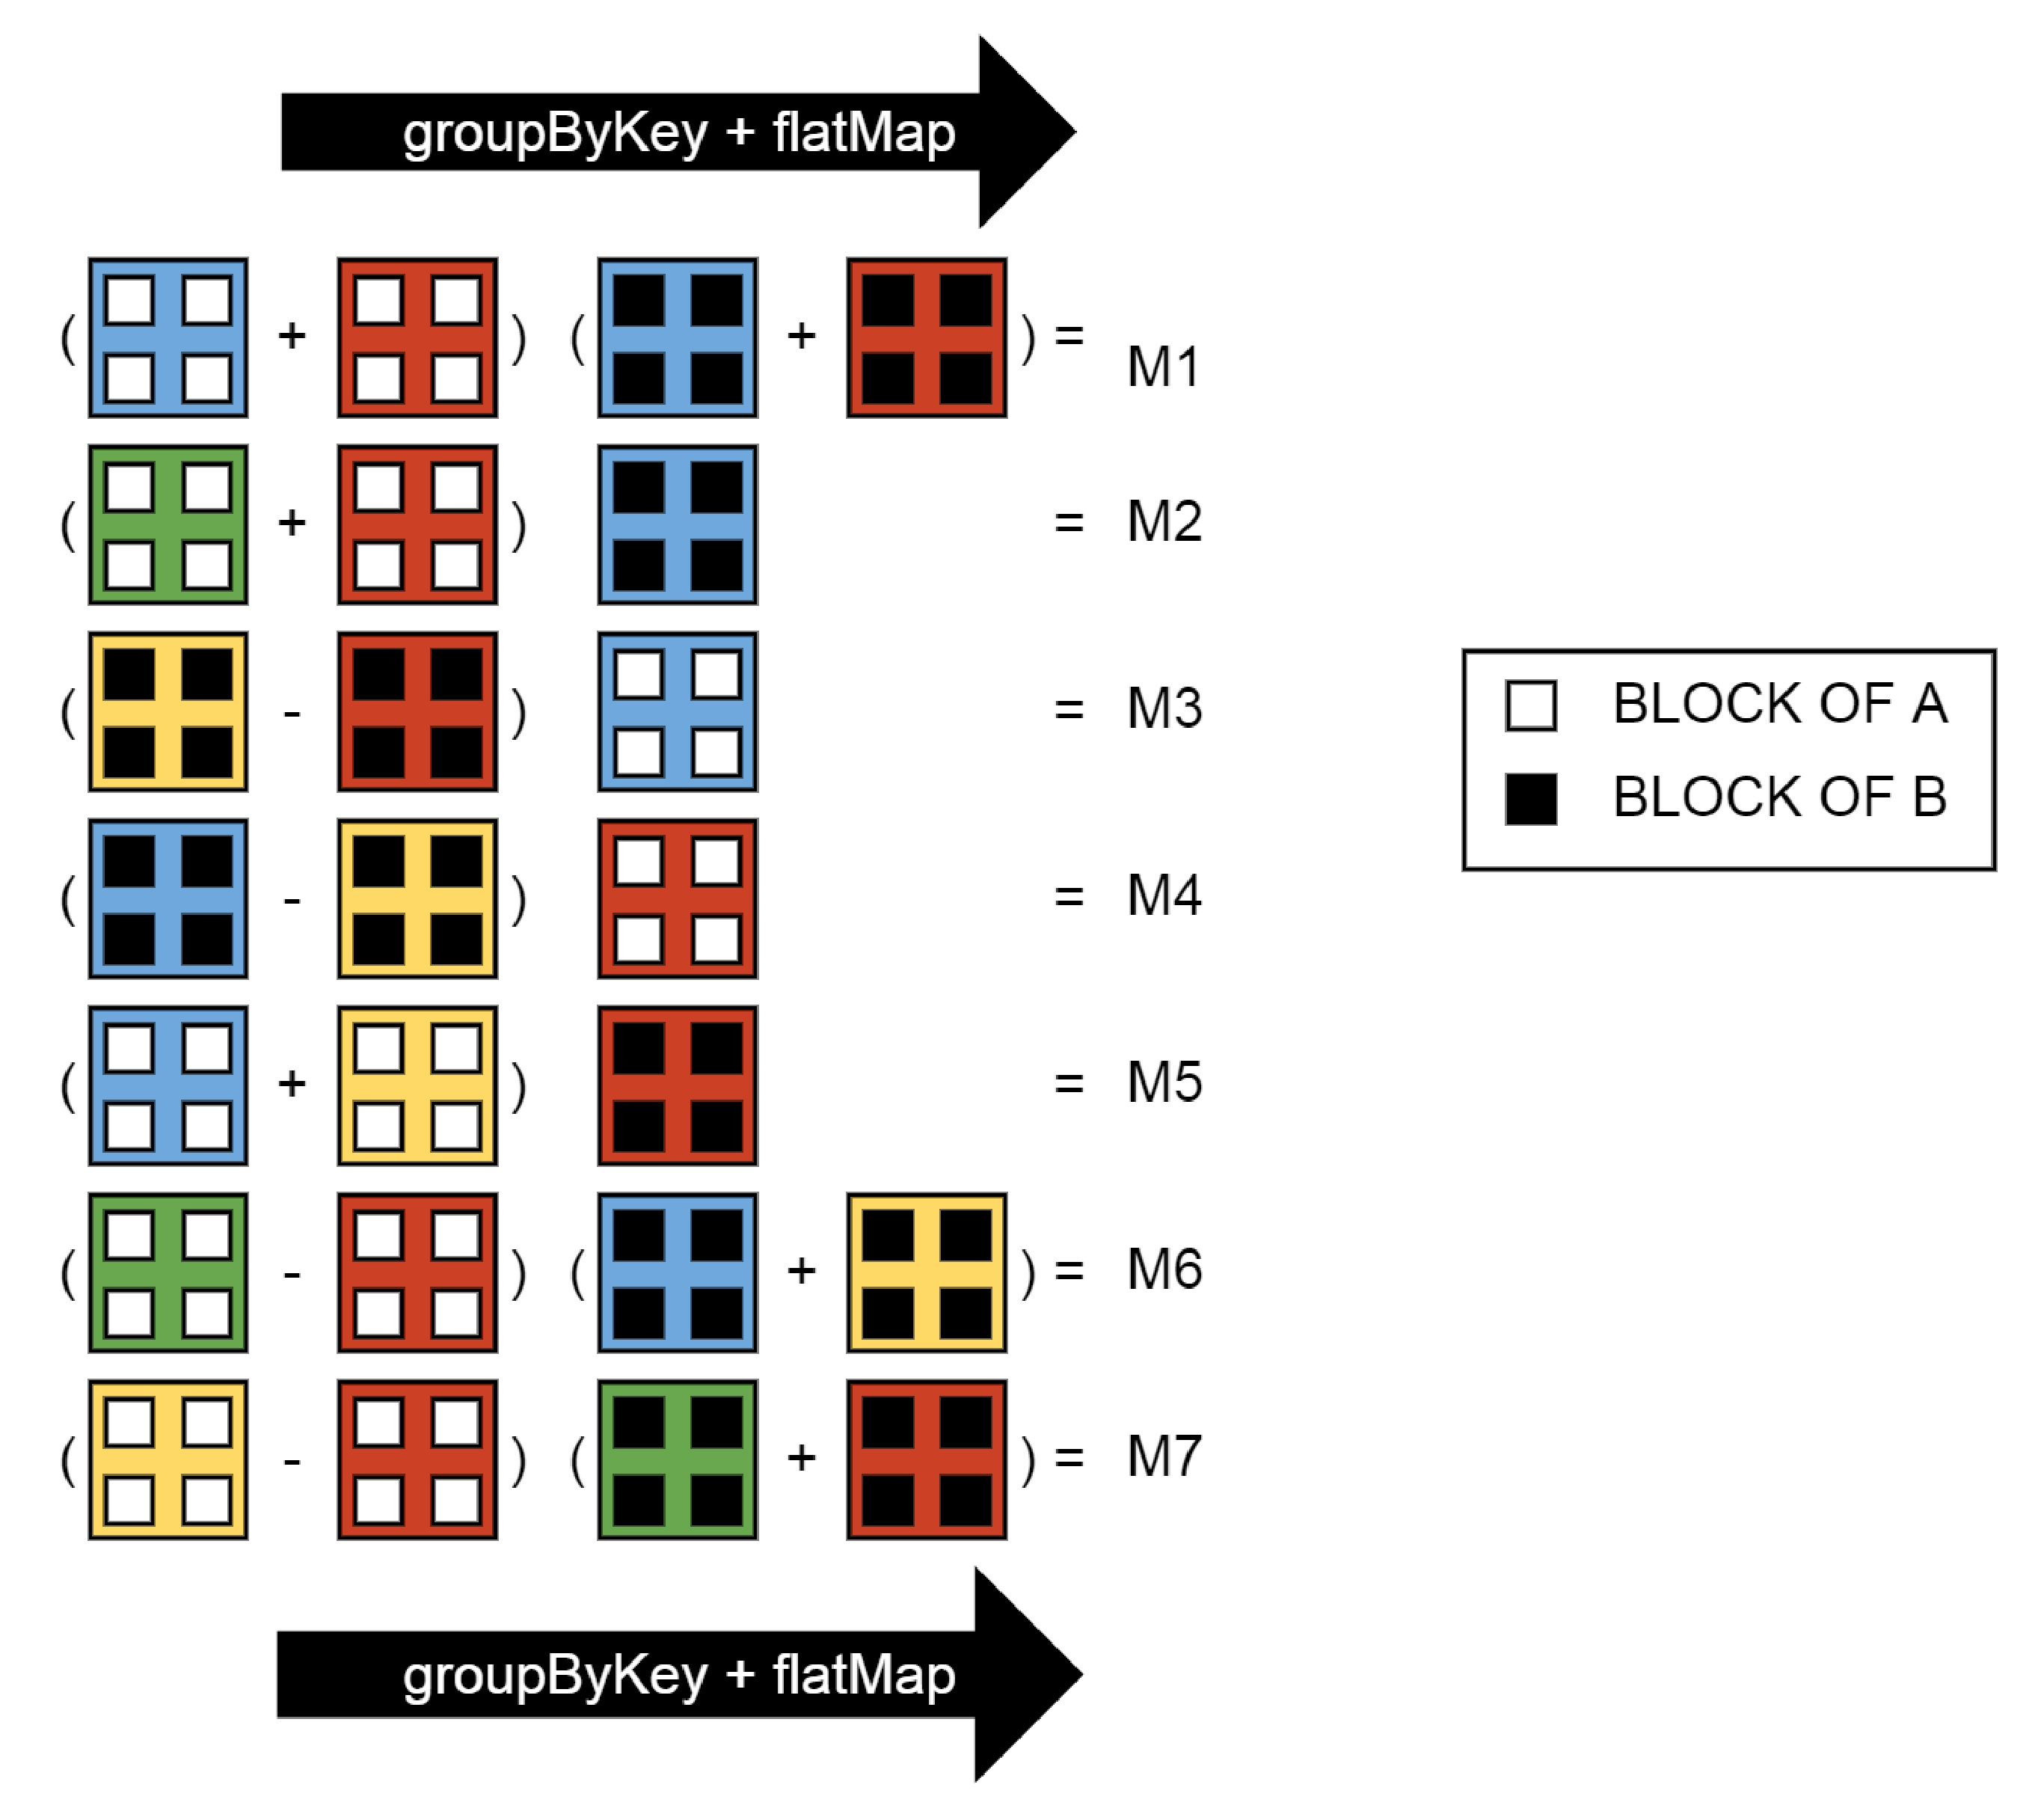
\includegraphics[scale=0.27]{images/add-sub.eps}
\caption{Addition and Subtraction of sub-matrices}
\label{fig:4}      
\end{figure}

%\subsubsection{Recursively divide the Sub-matrices}
Then we divide the intermediate blocks of the sub-matrices again by recursively calling the Strassen's method. Each time we go down the leaf of the execution tree, we divide the sub-matrices into smaller sub-matrices of size $\frac{n}{2}$. This process continues until it reaches the size of a block.

\subsubsection{Multiplication of Block index Matrices}
When the division reaches the size of user defined block size, the blocks are multiplied using serial MM algorithm. This is done using one \textit{mapToPair}, followed by one \textit{groupByKey} and one map function as shown in Algorithm \ref{alg:block-mul}. The \textit{mapToPair} function takes each block and returns a \textit{key-value} pair to group two potential blocks for multiplication. The \textit{groupByKey} groups two blocks and map function returns the multiplication of the two blocks. The keys in the \textit{mapToPair} function are chosen in such a way so that all the leaf index blocks are multiplied in parallel. We transform the leaf node block matrices to Breeze matrices to make the multiplication faster on a single node.

%%%%%%%%%%%%%%%%%%%%%%%%%%%%%%%%%%%%%%%% START OF BLOCK MM ALGORITHM %%%%%%%%%%%%%%%%%%%%%%%%%%%%%%%%%%%%%%%%%%%%%%%%%%%%%%%%%%%%%%%%%%%%%%
\begin{algorithm}
\SetAlgoLined
\SetKwFunction{procone}{MulBlockMat}
\SetKwProg{myproc}{Procedure}{}{}
\myproc{\procone{$RDD<Block> A$, $RDD<Block> B$}}{
    \tcc{Result contains RDD of blocks. Each block is the product of two matrix blocks residing in the same computer.}
    \KwResult{$RDD<Block> C$}
    \tcc{Make union of two input RDDs. Each block of the resulting RDD having a tag with string similar to $A|B, M_{1|2...|7},index$.}
    $RDD<Block> AunionB$ = $A$.union($B$)\;
    \tcc{Map each block to a (key,Block) pair. The key contains string $M_{1|2...|7},index$. Each Block contains a tag with string $A|B$.}
    $PairRDD<string, Block> firstMap$ = $AunionB$.mapToPair()\;
    \tcc{Group the blocks according to the key. For each key, this will group two blocks, one with block tag $A$ and another with $B$.}
    $PairRDD<string, iterable<Block>> group$ = $firstMap$.groupByKey()\;
    \tcc{Multiply two block matrix inside a single computer serially and return each Block to the resulting RDD.}
    $RDD<Block> C$ = $group$.map()\;
    \KwRet C\;    
}
\caption{Block Matrix Multiplication}
\label{alg:block-mul}
\end{algorithm}
%%%%%%%%%%%%%%%%%%%%%%%%%%%%%%%%%%%%%%% END OF BLOCK MATRIX MULTIPLICATION ALGORITHM %%%%%%%%%%%%%%%%%%%%%%%%%%%%%%%%%%%%%%%%%%%%%%%%%%%%%%%%%%%%%%%%%%%%%%%%%%%

\subsubsection{Combining the Sub-matrices}
In this step, the product matrix blocks of seven sub-matrices $M_{1}$ to $M_{7}$ are rearranged to produce a larger matrix. Combination phase occurs when the recursive call to Strassen's procedure returns. In each such return the size of the matrices becomes $2^{\frac{n}{2}}$ to $2^{n}$. Each such combine step is done in parallel. The combine step is shown in Algorithm \ref{alg:combine}.
\vspace{2mm}

%%%%%%%%%%%%%%%%%%%%%%%%%%%%%%%%%%%%%%%% START OF COMBINE ALGORITHM %%%%%%%%%%%%%%%%%%%%%%%%%%%%%%%%%%%%%%%%%%%%%%%%%%%%%%%%%%%%%%%%%%%%%%
\begin{algorithm}
\SetAlgoLined
\SetKwFunction{procone}{Combine}
\SetKwProg{myproc}{Procedure}{}{}
\myproc{\procone{$RDD<Block> BlockRDD$}}{
    \KwResult{$RDD<Block> C$}
    \tcc{Map each block to (key,Block) pair. Both the key and block mat-name contains string $M_{1|2...|7},index$. indexes are divided by 7 to blocks can be grouped of the same M sub-matrix.}
    $PairRDD<String,Block> firstMap$ = $BlockRDD$.map()\;
    \tcc{Group the blocks that comes from the same M sub-matrix}
    $PairRDD<string, iterable<Block>> group$ = $firstMap$.groupByKey()\;
    \tcc{combine the 7 sub-matrices of size n/2 to a single sub-matrix of size n having the same key}
    $RDD<Block> C$ = $group$.flatMap()\;
    \KwRet C\;    
}
\caption{Combine Phase}
\label{alg:combine}
\end{algorithm}
%%%%%%%%%%%%%%%%%%%%%%%%%%%%%%%%%%%%%%% END OF COMBINE ALGORITHM %%%%%%%%%%%%%%%%%%%%%%%%%%%%%%%%%%%%%%%%%%%%%%%%%%%%%%%%%%%%%%%%%%%%%%%%%%%

\section{Performance Modeling}
\label{sec:Performance_Modeling}
We will make an attempt to estimate the performance of Stark and state-of-the art \textit{Marlin} approach on a hypothetical exascale machine. We follow a methodology from \cite{gu2015efficient}, which gives runtime estimation based on the following parameters ---

\begin{itemize}
    \item $m$ = number of rows in matrix $A$
    \item $k$ = number of columns in matrix $A$
    \item $n$ = number of columns in matrix $B$
    \item $r$ = number of rows splits in matrix $A$
    \item $k$ = number of column splits in matrix $A$
    \item $n$ = number of column splits in matrix $B$
    \item $\left | A \right |$ = Size of matrix $A$
    \item $\left | B \right |$ = Size of matrix $B$
\end{itemize}

Therefore,

\begin{itemize}
    \item Total number of blocks in matrix $A$ = \textit{$rs$}
    \item Total number of blocks in matrix $B$ = \textit{$st$} and 
    \item Total number of blocks in both matrix $A$ and $B$ = \textit{$rs + st$}
\end{itemize}

\subsection{Cost Analysis of MLLib}
In this section we derive the cost of the MM subroutine of \textit{MLLib} package. As we have used block matrix data structure for \textit{Stark}, the same has been used for experimentation among four choices - \textit{RowMatrix}, \textit{IndexedRowMatrix}, \textit{CoordinateMatrix} and \textit{BlockMatrix}. In the pre-processing step we have transformed the input file to \textit{CoordinateMatrix}, and then converetd it into \textit{BlockMatrix}, a data structure synonymous to \textit{Stark's} block matrix structure. While converting to \textit{BlockMatrix}, we provided two parameters - \textit{rowsPerBlock} and \textit{colsPerBlock}. As each block is square, the value of these two parameters are same.

\begin{figure}		
	\centering
	\begin{tikzpicture}[squarednode/.style={rectangle, draw=blue!80, fill=blue!20, thin, minimum size=1.6em}, squarednodeTitle/.style={rectangle, draw=orange!80, fill=orange!20, thin, minimum size=1.6em}, background/.style={rectangle,fill=gray!14,inner sep=0.2cm,rounded corners=3mm}, node distance=1cm,->]
	
	%----------------------------Stage 1------------------------------------%
	\node[squarednode](stage11){\tiny textFile};
	\node[squarednode](stage21)[below of = stage11]{\tiny filter};
	\node[squarednode](stage31)[below of = stage21]{\tiny map};
	\node[squarednode](stage41)[below of = stage31]{\tiny map};
	
	\begin{pgfonlayer}{background}
	\node [background,fit= (stage11)(stage21)(stage31)(stage41)] (LargeBox) {};
	\end{pgfonlayer}
	
	\draw (stage11.south) -- (stage21.north);
	\draw (stage21.south) -- (stage31.north);
	\draw (stage31.south) -- (stage41.north);
	%------------------------------------------------------------------------%
	
	%----------------------------Stage 2------------------------------------%
	\node[squarednode](stage12)[right = 0.8cm of stage11]{\tiny textFile};
	\node[squarednode](stage22)[below of = stage12]{\tiny filter};
	\node[squarednode](stage32)[below of = stage22]{\tiny map};
	\node[squarednode](stage42)[below of = stage32]{\tiny map};
	
	\begin{pgfonlayer}{background}
	\node [background,fit= (stage12)(stage22)(stage32)(stage42)] (LargeBox) {};
	\end{pgfonlayer}
	
	\draw (stage12.south) -- (stage22.north);
	\draw (stage22.south) -- (stage32.north);
	\draw (stage32.south) -- (stage42.north);
	%------------------------------------------------------------------------%
	
	%----------------------------Stage 3------------------------------------%
	\node[squarednode](stage13)[right = 0.8cm of stage12]{\tiny groupByKey};
	\node[squarednode](stage23)[below of = stage13]{\tiny map};
	\node[squarednode](stage33)[below of = stage23]{\tiny flatMap};
	
	\begin{pgfonlayer}{background}
	\node [background,fit= (stage13)(stage23)(stage33)] (LargeBox) {};
	\end{pgfonlayer}
	
	\draw (stage13.south) -- (stage23.north);
	\draw (stage23.south) -- (stage33.north);
	%------------------------------------------------------------------------%
	
	%----------------------------Stage 4------------------------------------%
	\node[squarednode](stage14)[right = 0.8cm of stage13]{\tiny groupByKey};
	\node[squarednode](stage24)[below of = stage14]{\tiny map};
	\node[squarednode](stage34)[below of = stage24]{\tiny flatMap};
	
	\begin{pgfonlayer}{background}
	\node [background,fit= (stage14)(stage24)(stage34)] (LargeBox) {};
	\end{pgfonlayer}
	
	\draw (stage14.south) -- (stage24.north);
	\draw (stage24.south) -- (stage34.north);
	%------------------------------------------------------------------------%
	
	%----------------------------Stage 5------------------------------------%
	\node[squarednode](stage15)[right = 0.8cm of stage14]{\tiny coGroup};
	\node[squarednode](stage25)[below of = stage15]{\tiny flatMap};
	
	\begin{pgfonlayer}{background}
	\node [background,fit= (stage15)(stage25)] (LargeBox) {};
	\end{pgfonlayer}
	
	\draw (stage15.south) -- (stage25.north);
	%------------------------------------------------------------------------%
	
	%----------------------------Stage 6------------------------------------%
	\node[squarednode](stage16)[right = 0.8cm of stage15]{\tiny reduceByKey};
	\node[squarednode](stage26)[below of = stage16]{\tiny mapValues};
	
	\begin{pgfonlayer}{background}
	\node [background,fit= (stage16)(stage26)] (LargeBox) {};
	\end{pgfonlayer}
	
	\draw (stage16.south) -- (stage26.north);
	%------------------------------------------------------------------------%
	
	\draw (stage41.east) to [out=0, in=180](stage14.west);
	\draw (stage42.east) to [out=0, in=180](stage13.west);
	\draw (stage33.east) to [out=0, in=180](stage15.west);
	\draw (stage34.east) to [out=0, in=180](stage15.west);
	\draw (stage25.east) to [out=0, in=180](stage16.west);
	
	\node[squarednodeTitle](stage26)[above of = stage11, rounded corners=3mm]{\tiny Stage 1};
	\node[squarednodeTitle](stage26)[above of = stage12, rounded corners=3mm]{\tiny Stage 2};
	\node[squarednodeTitle](stage26)[above of = stage13, rounded corners=3mm]{\tiny Stage 3};
	\node[squarednodeTitle](stage26)[above of = stage14, rounded corners=3mm]{\tiny Stage 4};
	\node[squarednodeTitle](stage26)[above of = stage15, rounded corners=3mm]{\tiny Stage 5};
	\node[squarednodeTitle](stage26)[above of = stage16, rounded corners=3mm]{\tiny Stage 6};
	
	\end{tikzpicture}		
	\caption{Lineage graph of \textit{MLLib}}
	\label{fig:mllib-lineage}
\end{figure}

\begin{table}[h!]
	\caption{Stagewise cost analysis of MLLib}
	\label{tab:mllibCost}
	\begin{minipage}{\columnwidth}
		\begin{center}
			\begin{tabular}{llll}
				\toprule
				Stage-Step & Comp & Network & Parallelization Factor \\
				\toprule
				Stage 3-flatMap & $b^{3}$ & $NA$ & $min[b^{2}, cores]$ \\
				Stage 4-flatMap & $2b^{3}$ & $NA$ & $min[2b^{2}, cores]$ \\
				Stage 5-co-Group & $NA$ & $2b^{2}n^{2}$ & $min[b^{2}, cores]$ \\
				Stage 5-flatMap & $(\frac{n}{b})^{3}$ & $NA$ & $min[b^{2}, cores]$ \\
				Stage 6-reduceByKey & $NA$ & $\frac{n}{b}$ & $min[b^{2}, cores]$ \\
				\bottomrule
			\end{tabular}
		\end{center}
	\end{minipage}
\end{table}

Before multiplying, the method partitions the matrix blocks with unique \textit{partitionID} using \textit{GridPartitioner} approach. It partitions the input matrices in a grid structure and calculates four values - \textit{numRowBlocks} (number of row blocks), \textit{numColBlocks} (number of Column blocks), \textit{rowsPerPart} (number of row blocks per partition) and \textit{colsPerPart} (number of column blocks per partition). It then simulates the multiplication by calculating the destination \textit{partitionIDs} for each block so that only the required blocks is to be shuffled. This cuts the communication cost. For simulation, all the \textit{partitionIDs} needs to be collected at master node. Therefore, the \textit{IO} cost for this simulation part is

\begin{equation}
\begin{aligned}
IO_{simulation}&=(\frac{n}{b})^{2} + (\frac{n}{b})^{2}\\
&=2\times \frac{n^{2}}{b^{2}}
\end{aligned}
\end{equation}

We ignore the computation cost here, because the \textit{groupByKey} and \textit{map} steps are done on a single machine, the cost of which much less than the overall cost of the approach.

After simulating, two \textit{flatMap} steps are executed for two input matrices. These are shown in \textit{Stage 3} and \textit{Stage 4} of the lineage of \textit{MLLib} in Fig. \ref{fig:mllib-lineage}. The \textit{flatMap} is the actual block replication step where one block of $A$ is taken at a time and replicated as many times as it needs to be multiplied by other blocks of $B$. This value is the number of \textit{partitionIDs} of the blocks of $B$ , the input block should multiply which is equal to $b$. Therefore, total number of input blocks are $b^{2}$ and computation cost of \textit{Stage 3} and \textit{Stage 4} are

\begin{equation}
\begin{aligned}
Comp_{Stage3}&=b^{3}
\end{aligned}
\end{equation}

The parallelization factor for these two steps is

\begin{equation}
\begin{aligned}
PF_{Stage3}&=b^{2}
\end{aligned}
\end{equation}

After that, the actual shuffling takes place using co-group in \textit{Stage 5}. It groups the values associated to similar keys for both the $A$ and $B$ blocks, which is equal to 

\begin{equation}
\begin{aligned}
IO_{co-group}&=((numColPartB)\left | A \right |+(numRowPartA)\left | B \right |) \\
&=2b^{2}n^{2}
\end{aligned}
\end{equation}

The \textit{flatMap} step in \textit{Stage 5} computes the block level multiplication, the cost of which is 

\begin{equation}
\begin{aligned}
Comp_{flatMap}&=(\frac{n}{b})^{3} \\
\end{aligned}
\end{equation}

The parallelization factor of \textit{Stage 5} proportional to the total number of partitions of the product matrix, which is

\begin{equation}
\begin{aligned}
PF_{Stage5}&=b^{2}
\end{aligned}
\end{equation}

The \textit{reduceByKey} step of \textit{Stage 6} aggregates the multiplication terms in a group and add them. The \textit{IO} cost for this step is

\begin{equation}
\begin{aligned}
IO_{reduceByKey}&=\frac{n}{b}
\end{aligned}
\end{equation}

and the parallelization factor is same as above

\begin{equation}
\begin{aligned}
PF_{Stage6}&=b^{2}
\end{aligned}
\end{equation}

Therefore, the total cost of \textit{MLLib} is

\begin{equation}
\begin{aligned}
Cost_{MLLib}&=(IO_{Stage3}+IO_{Stage4}+IO_{Stage5}+Comp_{Stage5}+IO_{Stage6}) \\
&=\frac{b^{3}+b^{3}+2b^{2}n^{2}+(\frac{n}{b})^{3}+\frac{n}{b}}{min[b^{2}, cores]}
\end{aligned}
\end{equation}

%\begin{figure}[!h]
%\includegraphics[scale=0.5]{images/MLLib-Lineage.eps}    
%\caption{Lineage graph of \textit{MLLib}}\label{fig:MLLib-Lineage}
%\end{figure}

\subsection{Cost Analysis of Marlin}
Marlin job execution consists of $6$ stages as shown in Fig. \ref{fig:Marlin-Lineage}. However, \textit{Stage 1} and \textit{Stage 3} are part of the pre-processing steps. Also, the \textit{groupByKey} and \textit{mapValues} of \textit{Stage 2} and \textit{Stage 4} are not part of the actual multiplication job execution. Therefore, only \textit{flatMap} step of \textit{Stage 2} and \textit{Stage 4} and entire \textit{Stage 5} and \textit{Stage 6} are part of the actual execution.
A summary of the cost analysis is tabulated in Table \ref{tab:marlinCost}.

\begin{figure}[H]		
	\centering
	\begin{tikzpicture}[squarednode/.style={rectangle, draw=blue!80, fill=blue!20, thin, minimum size=1.6em}, squarednodeTitle/.style={rectangle, draw=orange!80, fill=orange!20, thin, minimum size=1.6em}, background/.style={rectangle,fill=gray!14,inner sep=0.2cm,rounded corners=3mm}, node distance=1cm,->]
	
	%----------------------------Stage 1------------------------------------%
	\node[squarednode](stage11){\tiny textFile};
	\node[squarednode](stage21)[below of = stage11]{\tiny map};
	\node[squarednode](stage31)[below of = stage21]{\tiny mapPartition};
	
	\begin{pgfonlayer}{background}
	\node [background,fit= (stage11)(stage21)(stage31)] (LargeBox) {};
	\end{pgfonlayer}
	
	\draw (stage11.south) -- (stage21.north);
	\draw (stage21.south) -- (stage31.north);
	%------------------------------------------------------------------------%
	
	%----------------------------Stage 2------------------------------------%
	\node[squarednode](stage12)[right = 0.8cm of stage11]{\tiny groupByKey};
	\node[squarednode](stage22)[below of = stage12]{\tiny mapPartition};
	\node[squarednode](stage32)[below of = stage22]{\tiny flatMap};
	
	\begin{pgfonlayer}{background}
	\node [background,fit= (stage12)(stage22)(stage32)] (LargeBox) {};
	\end{pgfonlayer}
	
	\draw (stage12.south) -- (stage22.north);
	\draw (stage22.south) -- (stage32.north);
	%------------------------------------------------------------------------%
	
	%----------------------------Stage 3------------------------------------%
	\node[squarednode](stage13)[right = 0.8cm of stage12]{\tiny textFile};
	\node[squarednode](stage23)[below of = stage13]{\tiny map};
	\node[squarednode](stage33)[below of = stage23]{\tiny mapPartition};
	
	\begin{pgfonlayer}{background}
	\node [background,fit= (stage13)(stage23)(stage33)] (LargeBox) {};
	\end{pgfonlayer}
	
	\draw (stage13.south) -- (stage23.north);
	\draw (stage23.south) -- (stage33.north);
	%------------------------------------------------------------------------%
	
	%----------------------------Stage 4------------------------------------%
	\node[squarednode](stage14)[right = 0.8cm of stage13]{\tiny groupByKey};
	\node[squarednode](stage24)[below of = stage14]{\tiny map};
	\node[squarednode](stage34)[below of = stage24]{\tiny flatMap};
	
	\begin{pgfonlayer}{background}
	\node [background,fit= (stage14)(stage24)(stage34)] (LargeBox) {};
	\end{pgfonlayer}
	
	\draw (stage14.south) -- (stage24.north);
	\draw (stage24.south) -- (stage34.north);
	%------------------------------------------------------------------------%
	
	%----------------------------Stage 5------------------------------------%
	\node[squarednode](stage15)[right = 0.5cm of stage14]{\tiny partitionBy};
	\node[squarednode](stage15D)[right = 0.1cm of stage15]{\tiny partitionBy};
	\node[squarednode](stage25)[below of = stage15D, xshift=-0.8cm]{\tiny join};
	\node[squarednode](stage35)[below of = stage25]{\tiny mapPartition};
	
	\begin{pgfonlayer}{background}
		\node [background,fit= (stage15)(stage15D)(stage25)(stage35)] (LargeBox) {};
	\end{pgfonlayer}
	
	\draw (stage15.south) -- (stage25.north);
	\draw (stage15D.south) -- (stage25.north);
	\draw (stage25.south) -- (stage35.north);
	%------------------------------------------------------------------------%
	
	%----------------------------Stage 6------------------------------------%
	\node[squarednode](stage16)[right = 0.5cm of stage15D]{\tiny reduceByKey};
	
	\begin{pgfonlayer}{background}
		\node [background,fit= (stage16)] (LargeBox) {};
	\end{pgfonlayer}
	%------------------------------------------------------------------------%
	
	\draw (stage31.east) to [out=0, in=180](stage12.west);
	\draw (stage32.east) to [out=0, in=180](stage15.west);
	\draw (stage33.east) to [out=0, in=180](stage14.west);
	\draw (stage34.east) to [out=0, in=180](stage15D.west);
	\draw (stage35.east) to [out=0, in=180](stage16.west);
	
	\node[squarednodeTitle](stage26)[above of = stage11, rounded corners=3mm]{\tiny Stage 1};
	\node[squarednodeTitle](stage26)[above of = stage12, rounded corners=3mm]{\tiny Stage 2};
	\node[squarednodeTitle](stage26)[above of = stage13, rounded corners=3mm]{\tiny Stage 3};
	\node[squarednodeTitle](stage26)[above of = stage14, rounded corners=3mm]{\tiny Stage 4};
	\node[squarednodeTitle](stage26)[above of = stage15, rounded corners=3mm, xshift=0.8cm]{\tiny Stage 5};
	\node[squarednodeTitle](stage26)[above of = stage16, rounded corners=3mm]{\tiny Stage 6};
	
	\end{tikzpicture}		
	\caption{Lineage graph of \textit{Marlin}}
	\label{fig:Marlin-Lineage}
\end{figure}

%\begin{figure}[!h]
%	\includegraphics[scale=0.5]{images/Marlin-Lineage.eps}    
%	\caption{Lineage graph for \textit{Marlin}}\label{fig:Marlin-Lineage}
%\end{figure}

\begin{table}[h!]
	\caption{Stagewise cost analysis of Marlin}
	\label{tab:marlinCost}
	\begin{minipage}{\columnwidth}
		\begin{center}
			\begin{tabular}{llll}
				\toprule
				Stage-Step & Comp & Network & Parallelization Factor \\
				\toprule
				Stage 2-flatMap & $2b^{3}$ & $2bn^{2}$ & $min[2b^{2}, cores]$ \\
				Stage 4-flatMap & $2b^{3}$ & $2bn^{2}$ & $min[2b^{2}, cores]$ \\
				Stage 5-Join & $NA$ & $bn^{2}$ & $min[b^{3}, cores]$ \\
				Stage 5-mapPartition & $n^{3}$ & $bn^{2}$ & $min[b^{3}, cores]$ \\
				Stage 6-reduceByKey & $NA$ & $bn^{2}$ & $min[b^{2}, cores]$ \\
				\bottomrule
			\end{tabular}
		\end{center}
	\end{minipage}
\end{table}

\subsubsection{Cost in Stage 2}
The only one step in \textit{Stage 2} that contributes to the cost is the \textit{flatMap} step. Below we derive the cost of \textit{flatMap} step.

\paragraph{Cost in flatMap Step}
In this step, each matrix block is taken as input and a list of matrix blocks is returned. Each block of matrix $A$ returns the number of columns of $B$ blocks and each block of $B$ returns the number of rows of $A$ blocks. Therefore, each block of total $rs$ blocks generates $t$ copies of $A$ blocks and each block of total $st$ blocks generates $r$ copies of $B$ blocks. Therefore, $IO$ cost can be derived as

\begin{equation}
    \begin{aligned}
        IO_{flatMap}&=(t\left | A \right |+r\left | B \right |) \\
        &=(r\times s\times t)+(r\times s\times t) \\
        &=2bn^{2}
    \end{aligned}
\end{equation}

The parallelization factor can be derived as

\begin{equation}
    \begin{aligned}
        PF_{flatMap}&=(rs+st) \\
        &=2b^{2}
    \end{aligned}
\end{equation}

We are ignoring the computing cost $Comp_{flatMap}$ cost in the \textit{flatMap} step as it is smaller than the $IO$ cost calculated above. Therefore, total cost in \textit{Stage 2} is

\begin{equation}
    \begin{aligned}
        Cost_{Stage 2}&=(2bn^{2}/min[2b^{2}, cores]) \\
        %&=n^{2}/b
    \end{aligned}
\end{equation}

\subsubsection{Cost in Stage 4}
The cost in \textit{Stage 4} is same as \textit{Stage 2} and therefore, total cost in \textit{Stage 4} is

\begin{equation}
    \begin{aligned}
        Cost_{Stage 2}&=(2bn^{2}/min[2b^{2}, cores]) \\
        %&=n^{2}/b
    \end{aligned}
\end{equation}

\subsubsection{Cost in Stage 5}
We have two steps in \textit{Stage 5}. They are \textit{join} and \textit{mapPartition}. We compute the \textit{IO} cost for \textit{join} and \textit{Comp} and \textit{IO} cost for \textit{mapPartition}.

\paragraph{Cost in Join Step}
In this step, the output from both the \textit{flatMap} steps are joined, so that related blocks stay together for the next \textit{mapPartition} step of \textit{Stage 5}. It shuffles only one matrix (either $A$ or $B$) through the network. Assuming only shuffling matrix $B$, the cost spending on the network communication can be derived as

\begin{equation}
    \begin{aligned}
        IO_{Join}&=(r\times \left | B \right |) \\
        &=(r\times s\times t) \\
        &=bn^{2}
    \end{aligned}
\end{equation}

At the same time, the programs reads blocks in matrix A locally, where the cost is much less than the networking cost and we can omit it in this step.

The parallelization factor is the number of multiplications done for each block times number of blocks in product matrix. Therefore,

\begin{equation}
    \begin{aligned}
        PF_{Join}&=(r\times s\times t) \\
        &=b^{3}
    \end{aligned}
\end{equation}

\paragraph{Cost in mapPartition Step}
In this step the MM are conducted locally. The computing cost of this step is

\begin{equation}
    \begin{aligned}
        Comp_{mapPartition}&=((m/b)\times (n/b)\times (k/b)) \\
        &=(n/b)^{3}
    \end{aligned}
\end{equation}

After the \textit{mapPartition} step the results blocks needs to be written to disks for the next shuffle phase. The \textit{IO} cost can be derived as

\begin{equation}
    \begin{aligned}
        IO_{mapPartition}&=(s\times \left | C \right |) \\
        &=(r\times s\times t) \\
        &=bn^{2}
    \end{aligned}
\end{equation}

The parallelization factor is the number of multiplications done for each block times number of blocks in product matrix. Therefore,

\begin{equation}
    \begin{aligned}
        PF_{mapPartition}&=(r\times s\times t) \\
        &=b^{3}
    \end{aligned}
\end{equation}

Therefore, total cost in \textit{Stage 5} is

\begin{equation}
    \begin{aligned}
        Cost_{Stage 5}&=(IO_{Join}/PF_{Join})+((Comp_{mapPartition}+IO_{mapPartition})/PF_{mapPartition}) \\
        &=(bn^{2}/min[b^{3}, cores])+((n^{3}+bn^{2})/min[b^{3}, cores]) \\
       % &=2+(n^{3}/bn^{2})
    \end{aligned}
\end{equation}

\subsubsection{Cost in Stage 6}
Cost in \textit{Stage 6} is the \textit{IO} cost in only step of this stage i.e. \textit{reduceByKey} step.

\paragraph{Cost in reduceByKey Step}
The \textit{IO} cost in this step is

\begin{equation}
    \begin{aligned}
        IO_{reduceByKey}&=(s\times \left | C \right |) \\
        &=(r\times s\times t) \\
        &=bn^{2}
    \end{aligned}
\end{equation}

In this step, the parallelization factor is the number of additions can be done in parallel which is equal to the number of blocks in the product matrix. Therefore,

\begin{equation}
    \begin{aligned}
        PF_{reduceByKey}&=(r\times t) \\
        &=b^{2}
    \end{aligned}
\end{equation}

Total cost in \textit{Stage 6} is

\begin{equation}
    \begin{aligned}
        Cost_{Stage 6}&=(IO_{reduceByKey}/PF_{reduceByKey}) \\
        &=(bn^{2}/min[b^{2}, cores]) \\
        %&=n^{2}/b
    \end{aligned}
\end{equation}

%Total cost in Marlin algorithm is

%\begin{equation}
%    \begin{aligned}
%        Cost_{Marlin}&=(Cost_{Stage 2}+Cost_{Stage 4}+Cost_{Stage 5}+Cost_{Stage 6}) \\
%        &=(n^{2}/b+n^{2}/b+2+n^{3}/bn^{2}+n^{2}/b) \\
%       &=(2+n/b+3n^{2}/b)
%    \end{aligned}
%\end{equation}

\subsection{Cost Analysis of Stark}
Unlike \textit{MLLib} and \textit{Marlin}, \textit{Stark} does not posses a constant number of stages. It depends on the number of recursive call to the algorithm. The algorithm can be divided into three main sections - \textit{Divide}, \textit{Multiply} and \textit{Combine}. \textit{Divide} section recursively divides the input matrices into seven sub-matrices and is done by three steps - \textit{flatMap}, \textit{groupByKey} and \textit{mapPartition}. The number of occurrences of these three steps depend on the number of recursive calls. The number of recursive calls are again equal to the logarithm of the number of partitions of the matrix. For example, for a $2^{p}\times 2^{p}$ matrix and $2^{q}\times 2^{q}$ matrix blocks, these three steps occur $\log_2(2^{p}/2^{q}) = (p-q)$ times. These three steps covers $(p-q)$ entire stages and first two of total three steps of an additional stage.

\begin{table}[h!]
	\caption{Stage-wise cost analysis of Stark}
	\label{tab:starkCost}
	\begin{minipage}{\columnwidth}
		\begin{center}
			\begin{tabular}{llll}
				\toprule
				Stage-Step & Comp & Network & P.F. \\
				\toprule
				Stage 1 to Stage $p-q$ \\ - map Divide & $\sum_{i=0}^{p-q-1}(7/2)^{i}(2b^{2})$ & $\sum_{i=0}^{p-q-1}3.(7/2)^{i}(2n^{2})$ & $min[7^{i}, cores]$ \\

				Stage 1 to Stage $p-q$ \\ - groupByKey Divide & $NA$ & $\sum_{i=0}^{p-q-1}3.(7/2)^{i}(2n^{2})$ & $min[7^{i}, cores]$ \\

				Stage 2 to \\ Stage $p-q+1$ \\ - flatMap Divide & $\sum_{i=1}^{p-q}(7/2)^{i}(2b^{2})$ & $NA$ & $min[7^{i}, cores]$ \\

				Stage $p-q+1$ \\ - map Leaf & $NA$ & $(7/4)^{p-q}(2n^{2})$ & $min[7^{p-q},cores]$ \\

				Stage $p-q+2$ \\ - groupByKey Leaf & $NA$ & $(7/4)^{p-q}(2n^{2})$ & $min[7^{p-q},cores]$ \\

				Stage $p-q+1$ \\ - map Leaf & $(7/4)^{p-q}(n^{3})$ & $NA$ & $min[7^{p-q},cores]$ \\

				Stage $p-q+2$ to \\ Stage $2p-2q+1$ \\ - map Combine & $\sum_{i=p-q}^{1}(7/4)^{i}(b^{2})$ & $\sum_{i=p-q}^{1}(7/2)^{i}(n^{2})$ & $min[7^{i}, cores]$ \\

				Stage $p-q+3$ to \\ Stage $2p-2q+2$ \\ - groupByKey Combine & $NA$ & $\sum_{i=p-q}^{1}(7/4)^{i}(n^{2})$ & $min[7^{i}, cores]$ \\

				Stage $p-q+3$ to \\ Stage $2p-2q+2$ \\ - flatMap Combine & $(12+8.(n)^{2}).4^{i-1}$ & $NA$ & $min[7^{i}, cores]$ \\
				\bottomrule
			\end{tabular}
		\end{center}
	\end{minipage}
\end{table}

  

\begin{figure}		
	\centering
	\begin{tikzpicture}[squarednode/.style={rectangle, draw=blue!80, fill=blue!20, thin, minimum size=1.6em}, squarednodeTitle/.style={rectangle, draw=orange!80, fill=orange!20, thin, minimum size=1.6em}, background/.style={rectangle,fill=gray!14,inner sep=0.2cm,rounded corners=3mm}, node distance=1cm,->]
	
	%----------------------------Stage 1------------------------------------%
	\node[squarednode](stage11){\tiny textFile};
	\node[squarednode](stage21)[below of = stage11]{\tiny map};
	\node[squarednode](stage31)[below of = stage21]{\tiny filter};
	\node[squarednode](stage41)[below of = stage31]{\tiny map};
	
	\begin{pgfonlayer}{background}
	\node [background,fit= (stage11)(stage21)(stage31)(stage41)] (LargeBox) {};
	\end{pgfonlayer}
	
	\draw (stage11.south) -- (stage21.north);
	\draw (stage21.south) -- (stage31.north);
	\draw (stage31.south) -- (stage41.north);
	%------------------------------------------------------------------------%
	
	%----------------------------Stage 2------------------------------------%
	\node[squarednode](stage12)[right = 0.5cm of stage11]{\tiny textFile};
	\node[squarednode](stage22)[below of = stage12]{\tiny map};
	\node[squarednode](stage32)[below of = stage22]{\tiny filter};
	\node[squarednode](stage42)[below of = stage32]{\tiny map};
	
	\begin{pgfonlayer}{background}
	\node [background,fit= (stage12)(stage22)(stage32)(stage42)] (LargeBox) {};
	\end{pgfonlayer}
	
	\draw (stage12.south) -- (stage22.north);
	\draw (stage22.south) -- (stage32.north);
	\draw (stage32.south) -- (stage42.north);
	%------------------------------------------------------------------------%
	
	%----------------------------Stage 3------------------------------------%
	\node[squarednode](stage13)[right = 0.5cm of stage12]{\tiny groupByKey};
	\node[squarednode](stage13D)[right = 0.1cm of stage13]{\tiny groupByKey};
	\node[squarednode](stage23)[below of = stage13]{\tiny mapValues};
	\node[squarednode](stage23D)[below of = stage13D]{\tiny mapValues};
	\node[squarednode](stage33)[below of = stage23]{\tiny map};
	\node[squarednode](stage33D)[below of = stage23D]{\tiny map};
	\node[squarednode](stage43)[below of = stage33, xshift = 0.9cm]{\tiny union};
	\node[squarednode](stage53)[below of = stage43]{\tiny flatmap};
	
	\begin{pgfonlayer}{background}
	\node [background,fit= (stage13)(stage13D)(stage23)(stage23D)(stage33)(stage33D)(stage43)(stage53)] (LargeBox) {};
	\end{pgfonlayer}
	
	\draw (stage13.south) -- (stage23.north);
	\draw (stage13D.south) -- (stage23D.north);
	\draw (stage23.south) -- (stage33.north);
	\draw (stage23D.south) -- (stage33D.north);
	\draw (stage33.south) to [out=270, in=180] (stage43.west);
	\draw (stage33D.south) to [out=270, in=0] (stage43.east);
	\draw (stage43.south) -- (stage53.north);
	%------------------------------------------------------------------------%
	
	%----------------------------Stage 4------------------------------------%
	\node[squarednode](stage14)[right = 0.5cm of stage13D]{\tiny groupByKey};
	\node[squarednode](stage24)[below of = stage14]{\tiny mapValues};
	\node[squarednode](stage34)[below of = stage24]{\tiny flatMap};
	\node[squarednode](stage44)[below of = stage34]{\tiny map};
	
	\begin{pgfonlayer}{background}
	\node [background,fit= (stage14)(stage24)(stage34)(stage44)] (LargeBox) {};
	\end{pgfonlayer}
	
	\draw (stage14.south) -- (stage24.north);
	\draw (stage24.south) -- (stage34.north);
	\draw (stage34.south) -- (stage44.north);
	%------------------------------------------------------------------------%
	
	%----------------------------Stage 5------------------------------------%
	\node[squarednode](stage15)[right = 0.5cm of stage14]{\tiny groupByKey};
	\node[squarednode](stage25)[below of = stage15]{\tiny mapValues};
	\node[squarednode](stage35)[below of = stage25]{\tiny flatMap};
	\node[squarednode](stage45)[below of = stage35]{\tiny map};
	
	\begin{pgfonlayer}{background}
	\node [background,fit= (stage15)(stage25)(stage35)(stage45)] (LargeBox) {};
	\end{pgfonlayer}
	
	\draw (stage15.south) -- (stage25.north);
	\draw (stage25.south) -- (stage35.north);
	\draw (stage35.south) -- (stage45.north);
	%------------------------------------------------------------------------%
	
	%----------------------------Stage 6------------------------------------%
	\node[squarednode](stage16)[right = 0.5cm of stage15]{\tiny groupByKey};
	\node[squarednode](stage26)[below of = stage16]{\tiny mapValues};
	\node[squarednode](stage36)[below of = stage26]{\tiny flatMap};
	
	\begin{pgfonlayer}{background}
	\node [background,fit= (stage16)(stage26)(stage36)] (LargeBox) {};
	\end{pgfonlayer}
	
	\draw (stage16.south) -- (stage26.north);
	\draw (stage26.south) -- (stage36.north);
	%------------------------------------------------------------------------%
	
	\node[squarednodeTitle](stage26)[above of = stage11, rounded corners=3mm]{\tiny Stage 1};
	\node[squarednodeTitle](stage26)[above of = stage12, rounded corners=3mm]{\tiny Stage 2};
	\node[squarednodeTitle](stage26)[above of = stage13, rounded corners=3mm,  xshift=0.8cm]{\tiny Stage 3};
	\node[squarednodeTitle](stage26)[above of = stage14, rounded corners=3mm]{\tiny Stage 4};
	\node[squarednodeTitle](stage26)[above of = stage15, rounded corners=3mm]{\tiny Stage 5};
	\node[squarednodeTitle](stage26)[above of = stage16, rounded corners=3mm]{\tiny Stage 6};
	
	\draw (stage41.east) to [out=0, in=180](stage13.west);
	\draw (stage42.east) to [out=0, in=180](stage13D.west);
	\draw (stage53.east) to [out=0, in=180](stage14.west);
	\draw (stage44.east) to [out=0, in=180](stage15.west);
	\draw (stage45.east) to [out=0, in=180](stage16.west);
	
	\end{tikzpicture}		
	\caption{Lineage graph of \textit{Stark}}
	\label{fig:Stark-Lineage}
\end{figure}

%\begin{figure}[!h]
%\includegraphics[scale=0.5]{images/Stark-Lineage.eps}    
%\caption{Lineage graph for \textit{Stark}}\label{fig:Stark-Lineage}
%\end{figure}

\textit{Multiply} section does the actual multiplication of leaf node matrix blocks. It consists of three steps - \textit{map}, \textit{groupByKey} and \textit{flatMap}. The first step occupy the last step of the previous stage and the next two steps occupy the first two steps of the next stage.

\textit{Combine} section combines the sub-matrices into a single matrix after the recursive call finishes. Like the first section, this section also consists of three steps - \textit{map}, \textit{groupByKey} and \textit{flatMap} and their occurrences are governed by the same logarithm function. Therefore, the total number of stages for a matrix of size of $2^{p}\times 2^{p}$ matrix and $2^{q}\times 2^{q}$ matrix blocks is 

\begin{equation}
    \begin{aligned}
        stages &= 2\log_2(2^{p}/2^{q}) + 2 \\
        &=2\log_22^{p-q} + 2 \\
        &=2(p-q)+2
    \end{aligned}
    \label{eq:Total_Stages}
\end{equation}

Fig. \ref{fig:Stark-Lineage} shows the lineage of \textit{Stark} when the value of $(p-q)$ is equal to $1$. For other scenarios, the lineage can be drawn according to equation \ref{eq:Total_Stages}. The cost analysis is summarized in Table \ref{tab:starkCost}.

\subsubsection{Cost Analysis in Divide Section}
As already stated, \textit{Divide} section consists of three steps - \textit{flatMap}, \textit{groupByKey} and \textit{mapPartition}. Each of the steps occurs $(p-q)$ times.

\paragraph{Cost Analysis of flatMap Step}
There are two types of cost associated with this step - computation cost and IO cost. The computation cost for a single \textit{flatMap} can be derived as

\begin{equation}
    \begin{aligned}
        Comp_{Single flatMap}&=(\left | A \right |+\left | B \right |) \\
        &=(rs+st) \\
        &=2b^{2}
    \end{aligned}
\end{equation}

As the recursion tree going down to the leaf nodes, the sub-matrix size starts to decrease whereas the number of nodes at each level increases $7$ times. Therefore, the total cost for this step for all the stages can be derived as

\begin{equation}
    \begin{aligned}
        Comp_{flatMap}&=\sum_{i=0}^{p-q-1}(7/2)^{i}(2b^{2}) \\        
    \end{aligned}
\end{equation}

The IO cost can be derived similarly as

\begin{equation}
    \begin{aligned}
        IO_{flatMap}&=\sum_{i=0}^{p-q-1}3.(7/2)^{i}(2n^{2}) \\        
    \end{aligned}
\end{equation}

As the program progresses the parallelization factor increases as $(7/4)^{i}(2b^{2})$ for $(i = 0, 1, 2, ..., (p-q-1))$.

\paragraph{Cost Analysis of groupByKey Step}
The network cost of this step is

\begin{equation}
    \begin{aligned}
        IO_{groupByKey}&=\sum_{i=0}^{p-q-1}3.(7/2)^{i}(2n^{2}) \\        
    \end{aligned}
\end{equation}

\paragraph{Cost Analysis of mapPartition Step}
The compute cost of \textit{mapPartition} step can be derived as

\begin{equation}
    \begin{aligned}
        Comp_{mapPartition}&=\sum_{i=1}^{p-q}(7/2)^{i}(2b^{2}) \\        
    \end{aligned}
\end{equation}

As the program progresses the parallelization factor increases as $(7)^{i}$ for $(i = 1, 2, ..., (p-q))$.

\subsubsection{Cost Analysis of Leaf Node Multiplication Section}
There are three steps for this section - \textit{mapPartition}, \textit{groupByKey} and \textit{map}. Each one occurs only once. The IO cost of \textit{mapPartition} step can be derived as

\begin{equation}
    \begin{aligned}
        IO_{mapPartition}&=(7/4)^{p-q}(2n^{2}) \\        
    \end{aligned}
\end{equation}

The \textit{IO} cost for \textit{groupByKey} step is

\begin{equation}
    \begin{aligned}
        IO_{groupByKey}&=(7/4)^{p-q}(2n^{2}) \\        
    \end{aligned}
\end{equation}

and the \textit{compute} cost for \textit{map} step is 

\begin{equation}
    \begin{aligned}
        Comp_{map}&=(7/4)^{p-q}(n^{3}) \\        
    \end{aligned}
\end{equation}

and the parallelization factor is $(7)^{p-q}$.

\subsubsection{Cost Analysis of Combine Section}
The \textit{Compute} cost for \textit{mapToPair} step can be derived as

\begin{equation}
    \begin{aligned}
        Comp_{mapPartition}&=\sum_{i=p-q}^{1}(7/4)^{i}(b^{2}) \\        
    \end{aligned}
\end{equation}

and \textit{IO} cost is same and parallelization factor is $(7)^{i}$ for $(i = (p-q), (p-q-1), ..., 1$.

The \textit{IO} cost for \textit{groupByKey} step is

\begin{equation}
    \begin{aligned}
        IO_{groupByKey}&=\sum_{i=p-q}^{1}(7/4)^{i}(n^{2}) \\        
    \end{aligned}
\end{equation}

and the parallelization factor is same as before.

The \textit{Compute} cost for \textit{flatMap} step is

\begin{equation}
    \begin{aligned}
       Comp_{flatMap}&=\sum_{i=p-q}^{1}(7)^{i-1}(7+b^{2}/4^{i}) \\        
    \end{aligned}
\end{equation}

Total cost for \textit{Stage 1}

\begin{equation}
    \begin{aligned}
       Cost_{Stage 1}&=\frac{6n^{2}}{min[1, cores]}        
    \end{aligned}
\end{equation}

Total Cost for \textit{Stage 2} to \textit{Stage $(p-q)$}

\begin{equation}
    \begin{aligned}
       Cost_{Stage 2 to (p-q)}&=\sum_{i=0}^{p-q-2}\frac{3.(7/2)^{i}.(2n^{2})}{min[(7/4)^{i}\times 2b^{2}, cores]}+\sum_{i=0}^{p-q-1}\frac{3.(7/2)^{i}.(2n^{2})}{min[7^{i+1}, cores]} \\
       &+\sum_{i=1}^{p-q}\frac{(7/2)^{i}(2b^{2})}{min[7^{i+1}, cores]}+\frac{(7/4)^{p-q}(2n^{2})}{min[7^{p-q}, cores]}
    \end{aligned}
\end{equation}

Total Cost for \textit{Stage (p-q+1)}

\begin{equation}
    \begin{aligned}
       Cost_{Stage (p-q+1)}&=\frac{(7/4)^{p-q}(2n^{2})}{min[7^{p-q}, cores]}+\frac{(7/4)^{p-q}(n^{3})}{min[7^{p-q}, cores]}+\frac{(7/4)^{p-q}(b^{2})}{min[7^{i}, cores]}
    \end{aligned}
\end{equation}

Total cost for \textit{Stage (p-q+1)} to \textit{Stage (2(p-q)+1)}

\begin{equation}
    \begin{aligned}
       Cost_{Stage (p-q+2) to (2(p-q)+1)}&=\sum_{i=p-q-1}^{1}\frac{(7/4)^{i}(n^{2})}{min[7^{i}, cores]}+\sum_{i=p-q-1}^{1}\frac{7^{i-1}(7+b^{2}/4^{i})}{min[7^{i}, cores]}\\&+\sum_{i=p-q-1}^{1}\frac{(7/4)^{i}(b^{2})}{min[7^{i}, cores]}
    \end{aligned}
\end{equation}

Total cost for \textit{Stage 2(p-q)+2}

\begin{equation}
    \begin{aligned}
       Cost_{Stage (2(p-q)+2)}&=\frac{(7/4)n^{2}}{min[7, cores]}+\frac{(12+8n^{2})\times 4^{i-1}}{min[7, cores]}
    \end{aligned}
\end{equation}

%Total cost for Stark is
%
%\begin{equation}
%    \begin{aligned}
%       Cost_{Strassen's}&=3.(n/b)^{2}+3.(n/b)^{2}\sum_{i=0}^{p-q-2}(1/2)^{i}+(6n^{2}+b^{2})/7+\sum_{i=0}^{p-q-1}(1/2)^{i}+n^{2}/2^{p-q-1}\\
%       &+(n^{3}+2n^{2}+b^{2})/4^{p-q}+\sum_{i=0}^{p-q-1}(1/4)^{i}(n^{2}+8.b^{2}/7)+1+(bn/2)^{2}+7
%    \end{aligned}
%\end{equation}

\section{Experiments}
\label{sec:Experimental-Evaluation}
In this section, we perform experiments to evaluate the execution efficiency of \textit{Stark} comparing it with \textit{Marlin} and \textit{MLLib} and scalability of the algorithm compared to ideal scalability. First, we select the fastest execution time among different partition size for each approach and compare them. Second, we conduct a series of experiments to individually evaluate the effect of partition size and matrix size of each competing approach. At last, we evaluate the scalability of \textit{Stark}.

\subsection{Test Setup}
All the experiments are carried out on a dedicated cluster of 3 nodes. Software and hardware specifications are summarized in Table \ref{tab:test-setup}. Here NA means not applicable.

\begin{table}[h!]
	\caption{Summary of Test setup components specifications}
	\label{tab:test-setup}
	\begin{minipage}{\columnwidth}
		\begin{center}
			\begin{tabular}{lll}
				\toprule
				Component Name & Component Size & Specification \\
				\toprule
				Processor & 2 & Intel Xeon 2.60 GHz \\
				Core & 6 per processor & NA \\
				Physical Memory & 132 GB & NA \\
				Ethernet & 14 Gb/s & Infini Band \\
				OS & NA & CentOS 5 \\
				File System & NA & Ext3 \\
				Apache Spark & NA & 1.6.0 \\
				Apache Hadoop & NA & 2.6.0 \\
				%jBlas & NA & 1.2.4 \\
				Java & NA & 1.7.0 update 79 \\
				\bottomrule
			\end{tabular}
		\end{center}
	\end{minipage}
\end{table}

For block level multiplications \textit{Stark} uses Breeze, a single node low-level linear algebra library. Breeze provides Java APIs to \textit{Stark} through Spark, and it calls C/Fortran-implemented native library, such as BLAS, to execute the linear algebra computation through the Java Native Interface (JNI). We have tested the algorithms on matrices with increasing cardinality from $(16 \times 16)$ to $(16384 \times 16384)$. All of these test matrices have been generated randomly using Java Random class. The elements of the matrices are of double-precision $64$-bit IEEE $754$ floating point type.

%Each node has 2 Intel Xeon 2.60 GHz processors, 6 cores per processor, 132 GB of physical memory, 15 TB hard disk space. The nodes are connected with \color{red} 1 Gb/s \color{black} Ethernet. All the nodes are run on CentOS 5 operating system and Ext3 file system. Apache Spark 1.6.0 is used for our implmentation and we employ jBlas 1.2.4 for native linear algebra library support for Java. The underlying Hadoop version is 2.6.0 and the Java version is 1.7.0 update 79. 

\subsubsection{Resource Utilization Plan}

%\color{red}
%Merge with above section\\
%spark configuration\
%Main points are:
%there is no thrashing\\
%We ensure that none of the cases the jobs had to be restarted\\
%\color{black}

While running the jobs in the cluster, we customize three parameters --- the number of executors, the executor memory and the executor cores. We wanted a fair comparison among the competing approaches and therefore, we ensured jobs should not experience \textit{thrashing} and none of the cases tasks should fail and jobs had to be restarted. For this reason, we restricted ourselves to choose the parameters value which provides good utilization of cluster resources and mitigating the chance of task failures. By experimentation we found that, keeping executor memory as $50$ GB ensures successful execution of jobs without \textit{``out of memory''} error or any task failures for all the competing approaches. This includes the small amount of overhead to determine the full request to YARN for each executor which is equal to $3.5$ GB. Therefore, the executor memory is $46.5$ GB. Though the physical memory of each node is $132$ GB, we keep only $100$ GB as YARN resource allocated memory for each node. Therefore, the total physical memory for job execution is $100$ GB resulting $2$ executors per node and a total $6$ executors.  We reserve, $1$ core for operating system and hadoop daemons. Therefore, available total core is $11$. This leaves $5$ cores for each executor. We used these values of the run time resource parameters in all the experiments except the scalability test, where we have test the approach with varied number of executors. The resource utilization plan is summarized in Table \ref{tab:resourceUtil}.

\begin{table}[h!]
	\caption{Resource Utilization Plan for Efficiency Experiments of Stark with \textit{MLLib} and \textit{Marlin}}
	\label{tab:resourceUtil}
	\begin{minipage}{\columnwidth}
		\begin{center}
			\begin{tabular}{lll}
				\toprule
				Component Name & Component Size \\
				\toprule
				Executors & 5 \\
				Executor Cores & 5 \\
				Executor Memory & 40GB \\
				YARN Memory & 100GB \\
				\bottomrule
			\end{tabular}
		\end{center}
	\end{minipage}
\end{table}

\subsection{Efficiency}

\subsubsection{Practical Utility of Stark: Comparison with state-of-the-art distributed systems}
In this section, we examine the performance of Stark with other Spark based distributed MM approaches i.e. \textit{Marlin} and \textit{MLLib}. We report the running time of the competing approaches with increasing matrix size. We take the best running time (fastest) among all the running time taken for different block sizes. The experimental results are shown in Fig. \ref{fig:Fastest-Running-Time}. It can be seen that performance of \textit{Stark} is faster than the \textit{Marlin} and \textit{MLLib}. Also, the performance is increased as matrix size is increased from $(4096\times 4096)$ to $(16384\times 16384)$. %Table \ref{tab:Running-Time-Tab} provides detailed report on the running time of the approaches for all matrix sizes and block sizes. \textcolor{red}{[Should I provide the reason why it is faster in all matrix sizes and block sizes.]} From the table it can be seen that \textit{Stark} outperforms others for any matrix size and any block size.

\begin{figure}
	\centering		
		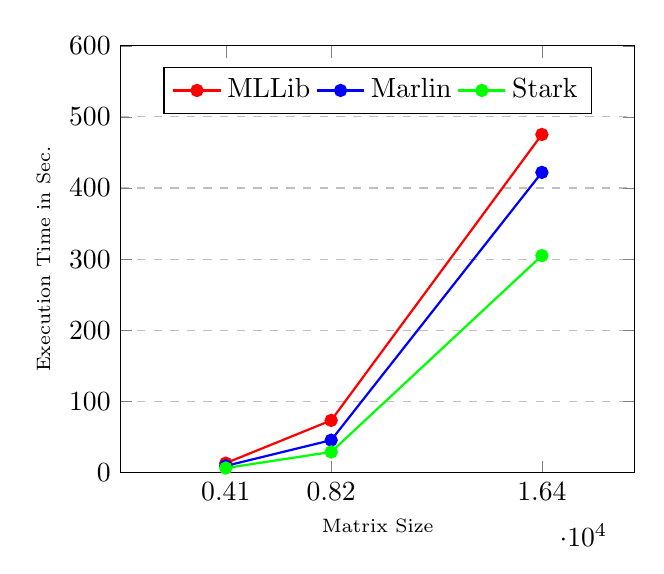
\begin{tikzpicture}
		\begin{axis}[
		height=7cm,
		%title={Temperature dependence of CuSO$_4\cdot$5H$_2$O solubility},
		xlabel={},
		ylabel={},
		xmin=0, xmax=20000,
		ymin=0, ymax=600,
		xtick={4096,8192,16384},
		ytick={0,100,200,300,400,500,600},
		every axis plot/.append style={thick},
		xlabel={\scriptsize Matrix Size},
		ylabel={\scriptsize Execution Time in Sec.},
		legend style={at={(0.5,0.95)},
		anchor=north,legend columns=-1},
		ymajorgrids=true,
		grid style=dashed,
		]
		
		\addplot[
		color=red,
		mark=*,
		]
		coordinates {
			(4096,13.1)(8192,73.2)(16384,475.3)
		};
		
		\addplot[
		color=blue,
		mark=*,
		]
		coordinates {
			(4096,9.2)(8192,45.4)(16384,422)
		};
	
		\addplot[
		color=green,
		mark=*,
		]
		coordinates {
			(4096,6.2)(8192,28.8)(16384,305)
		};
	
		\legend{MLLib, Marlin, Stark}
		
		\end{axis}
		\end{tikzpicture}
	\caption{Fastest running time of three systems among different block sizes}\label{fig:Fastest-Running-Time}
\end{figure}

\subsubsection{Variation with matrix size}
In this experiment we compare the running time for increasing matrix size. For each matrix size we compare the running time for increasing partition size. Fig. \ref{fig:Running-Time-Size} shows the comparison.

\begin{figure}[!ht]
	\begin{subfigure}[t]{.35\textwidth}
		\begin{tikzpicture}
		\begin{axis}[
		xmin=0,
		xmax=17,
		xtick={2,4,8,16},
		ytick={10,20,30,40,50},
		x tick label style={/pgf/number format/1000 sep=},
		xlabel={\tiny Partition Size},
		ylabel={\tiny Execution Time in Sec.},
		legend style={at={(0.74,1.5)},anchor=north},
		width=\textwidth,
		]
		\addplot coordinates {(2,43.6) (4,35.5) (8,21.2) (16,13.1)};
		\addlegendentry{\tiny MLLib}
		\addplot coordinates {(2,15) (4,11.5) (8,9.2) (16,14.2)};
		\addlegendentry{\tiny Marlin}
		\addplot coordinates {(2,21.8) (4,12) (8,10.2) (16,15.1)};
		\addlegendentry{\tiny Stark}
		\end{axis}
		\end{tikzpicture}
		\caption{$4096\times 4096$},
	\end{subfigure}%
	\begin{subfigure}[t]{.35\textwidth}
		\begin{tikzpicture}
		\begin{axis}[
		xmin=0,
		xmax=17,
		xtick={2,4,8,16},
		ytick={50,100,150,200,250,300,350},
		x tick label style={/pgf/number format/1000 sep=},
		xlabel={\tiny Partition Size},
		ylabel={\tiny Execution Time in Sec.},
		legend style={at={(0.74,1.5)},anchor=north},
		width=\textwidth,
		]
		\addplot coordinates {(2,273) (4,106.6) (8,83.3) (16,73.2)};
		\addlegendentry{\tiny MLLib}
		\addplot coordinates {(2,193) (4,77) (8,45.4) (16,56.3)};
		\addlegendentry{\tiny Marlin}
		\addplot coordinates {(2,224) (4,74) (8,45) (16,40.8)};
		\addlegendentry{\tiny Stark}
		\end{axis}
		\end{tikzpicture}
		\caption{$8192\times 8192$}
	\end{subfigure}%
	\begin{subfigure}[t]{.35\textwidth}
		\begin{tikzpicture}
		\begin{axis}[
		xmin=0,
		xmax=17,
		xtick={2,4,8,16},
		ytick={200,400,600,800,1000},
		x tick label style={/pgf/number format/1000 sep=},
		xlabel={\tiny Partition Size},
		ylabel={\tiny Execution Time in Sec.},
		legend style={at={(0.74,1.5)},anchor=north},
		width=\textwidth,
		]
		\addplot coordinates {(4,1028) (8,535) (16,475.3)};
		\addlegendentry{\tiny MLLib}
		\addplot coordinates {(4,741) (8,447) (16,422)};
		\addlegendentry{\tiny Marlin}
		\addplot coordinates {(4,631) (8,326) (16,305)};
		\addlegendentry{\tiny Stark}
		\end{axis}
		\end{tikzpicture}
		\caption{$16384\times 16384$}
	\end{subfigure}%
	\caption{Comparing running time of Stark, Marlin and MLLib for matrix size $(4096\times 4096)$, $(8192\times 8192)$, $(16384\times 16384)$ for increasing partition size}\label{fig:Running-Time-Size}
\end{figure}

The results show that, as matrix size increases the execution time of Stark grows slowly than others providing faster execution at $16$ partition size in $8192\times 8192$ and all the partition sizes in $16384\times 16384$. Moreover, as the partition size increases the difference in running time also increases. 

\subsubsection{Comparison with state of the art single node systems}
%\color{red}
%Write the blocksize search range\\
%Repeat that number fo executors is constant even for small size matrices.
%\color{black}
The second experiment (Table \ref{tab:CompWithSingleNode}) examines how the runtime improves if we use Stark on the cluster compared to the serial MM on a single node having similar configuration of a single node in the cluster. The intension of this experiment is to provide a demonstration of how well our approach performs when robust linear algebraic libraries are run on a single node with equal power and specifications. To present such comparison, we use Colt \cite{colt} and JBlas \cite{jblas}, two linear algebra routines implementing MM algorithm having optimized code. Colt is a set of open source libraries for high performance technical computing in Java. On the other hand, JBlas is a fast linear algebra library for Java based on BLAS and LAPACK. We use the parallel version of Colt library, named ParallelColt \cite{wendykier2010parallel} which uses threads automatically when computations are done on a machine with multiple CPUs. Additionally, we use two other variations of single node serial MM algorithm --- the three loop na\"{i}ve approach and the single node Strassen's MM algorithm. We use \textit{NA} when the execution time is more than reasonable time i.e. more than $1$ hour. 

\begin{table}[h!]
\caption{Performance comparison of five systems with increasing matrix size (The unit of execution time is second)}
\label{tab:CompWithSingleNode}
\begin{minipage}{\columnwidth}
\begin{center}
\begin{tabular}{llllll}
\toprule
    Matrix & SN & SS & Colt & JBlas & Stark \\
 	\toprule
    %$16 \times 16$ & $<1$ & $<1$ & $<1$ & $<1$ & 4 \\
    %$32 \times 32$ & $<1$ & $<1$ & $<1$ & $<1$ & 4 \\
    %$64 \times 64$ & $<1$ & $<1$ & $<1$ & $<1$ & 4 \\
    %$128 \times 128$ & $<1$ & $<1$ & $<1$ & $<1$ & 4 \\
    %$256 \times 256$ & $<1$ & $<1$ & $<1$ & $<1$ & 4 \\
    $512 \times 512$ & $<1$ & $<1$ & $<1$ & $<1$ & 5 \\
    $1024 \times 1024$ & 15 & 2 & 1 & $<1$ & 6 \\
    $2048 \times 2048$ & 177 & 14 & 13 & 2 & 9 \\
    $4096 \times 4096$ & 2112 & 100 & 135 & 16 & 6.2 \\
    $8192 \times 8192$ & NA & 394 & 1163 & 119 & 28.8 \\
    $16384 \times 16384$ & NA & 2453 & NA & 862 & 305 \\
\bottomrule
\end{tabular}
\end{center}
\end{minipage}
\end{table}

For each matrix of size $2^{n}\times 2^{n}$, we take the running time increasing the block size from $2$ to $2^{\frac{n}{2}}\times 2^{\frac{n}{2}}$. We take the fastest running time for each matrix size and report it. The results shows that \textit{Stark} outperforms others with a very substantial margin. 

\subsubsection{Variation with partition size}
In this experiment, we show that there is an optimal partition size for each of the competing method. To demonstrate that we generate three scenarios for each method. We increase matrix size from $(4096\times 4096)$ to $(16384\times 16384)$ respectively and increase partition size from 4 to 16 in each scenario. Fig. \ref{fig:Running-Time-Partition-MLLib}, Fig. \ref{fig:Running-Time-Partition-Marlin} and Fig. \ref{fig:Running-Time-Partition-Stark} show scenarios respectively.

\begin{figure}[!ht]
	\begin{subfigure}[t]{.35\textwidth}
		\begin{tikzpicture}
		\begin{axis}[
		xmin=0,
		xmax=17,
		xtick={2,4,8,16},
		ytick={10,20,30,40,50,60,70},
		x tick label style={/pgf/number format/1000 sep=},
		xlabel={\tiny Partition Size},
		ylabel={\tiny Execution Time in Sec.},
		legend style={at={(0.5,1.5)},anchor=north},
		width=\textwidth,
		]
		\addplot coordinates {(2,65.52) (4,32.65) (8,0.0718) (16,0.0393)};
		\addlegendentry{Theoretical}
		\addplot coordinates {(2,43.6) (4,35.5) (8,21.2) (16,13.1)};
		\addlegendentry{Experimantal}
		\end{axis}
		\end{tikzpicture}
		\caption{$4096\times 4096$},
	\end{subfigure}%
	\begin{subfigure}[t]{.35\textwidth}
		\begin{tikzpicture}
		\begin{axis}[
		xmin=0,
		xmax=17,
		xtick={2,4,8,16},
		ytick={50,100,150,200,250,300},
		x tick label style={/pgf/number format/1000 sep=},
		xlabel={\tiny Partition Size},
		ylabel={\tiny Execution Time in Sec.},
		legend style={at={(0.5,1.5)},anchor=north},
		width=\textwidth,
		]
		\addplot coordinates {(2,115.02) (4,14.59) (8,4.80) (16,2.54)};
		\addlegendentry{Theoretical}
		\addplot coordinates {(2,275) (4,95.6) (8,85.3) (16,73.2)};
		\addlegendentry{Experimantal}
		\end{axis}
		\end{tikzpicture}
		\caption{$8192\times 8192$}
	\end{subfigure}%
	\begin{subfigure}[t]{.35\textwidth}
		\begin{tikzpicture}
		\begin{axis}[
		xmin=0,
		xmax=17,
		xtick={2,4,8,16},
		ytick={225,450,675,900,1125},
		x tick label style={/pgf/number format/1000 sep=},
		xlabel={\tiny Partition Size},
		ylabel={\tiny Execution Time in Sec.},
		legend style={at={(0.5,1.5)},anchor=north},
		width=\textwidth,
		]
		\addplot coordinates {(2,856.51) (4,100.35) (8,32.65) (16,16.86)};
		\addlegendentry{Theoretical}
		\addplot coordinates {(4,1028) (8,535) (16,475.3)};
		\addlegendentry{Experimantal}
		\end{axis}
		\end{tikzpicture}
		\caption{$16384\times 16384$}
	\end{subfigure}%
	\caption{Comparing theoretical and experimental running time of MLLib for matrix size $(4096\times 4096)$, $(8192\times 8192)$, $(16384\times 16384)$ for increasing partition size}\label{fig:Running-Time-Partition-MLLib}
\end{figure}

It is clearly seen that MLLib execution time (experimental) entirely matches with the theoretical one. Both are decreasing with increasing partition size. The costliest part of MLLib is the computation of multiplication of block matrices, which is $((n/b)^{3}/min[b,25])$. For partition size $b=2$ and $4$ the factor decreases drastically because, the denominator becomes $b^{3}$. After that, the parallelization factor becomes constant which is $25$, the number of cores designated for the spark job. So, the denominator $b$ affects the execution time and thus it decreases gradually.

\begin{figure}[!ht]
	\begin{subfigure}[t]{.35\textwidth}
		\begin{tikzpicture}
		\begin{axis}[
		xmin=0,
		xmax=17,
		xtick={2,4,8,16},
		ytick={2,4,6,8,10,12,14,16},
		x tick label style={/pgf/number format/1000 sep=},
		xlabel={\tiny Partition Size},
		ylabel={\tiny Execution Time in Sec.},
		legend style={at={(0.5,1.5)},anchor=north},
		width=\textwidth,
		]
		\addplot coordinates {(2,8.88) (4,2.92) (8,3.07) (16,3.39)};
		\addlegendentry{Theoretical}
		\addplot coordinates {(2,15) (4,11.5) (8,9.2) (16,14.2)};
		\addlegendentry{Experimantal}
		\end{axis}
		\end{tikzpicture}
		\caption{$4096\times 4096$},
	\end{subfigure}%
	\begin{subfigure}[t]{.35\textwidth}
		\begin{tikzpicture}
		\begin{axis}[
		xmin=0,
		xmax=17,
		xtick={2,4,8,16},
		ytick={50,100,150,200,250,300,350},
		x tick label style={/pgf/number format/1000 sep=},
		xlabel={\tiny Partition Size},
		ylabel={\tiny Execution Time in Sec.},
		legend style={at={(0.5,1.5)},anchor=north},
		width=\textwidth,
		]
		\addplot coordinates {(2,69.89) (4,22.69) (8,23.28) (16,24.57)};
		\addlegendentry{Theoretical}
		\addplot coordinates {(2,193) (4,77) (8,45.4) (16,56.3)};
		\addlegendentry{Experimantal}
		\end{axis}
		\end{tikzpicture}
		\caption{$8192\times 8192$}
	\end{subfigure}%
	\begin{subfigure}[t]{.35\textwidth}
		\begin{tikzpicture}
		\begin{axis}[
		xmin=0,
		xmax=17,
		xtick={2,4,8,16},
		ytick={100,200,300,400,500,600,700,800},
		x tick label style={/pgf/number format/1000 sep=},
		xlabel={\tiny Partition Size},
		ylabel={\tiny Execution Time in Sec.},
		legend style={at={(0.5,1.5)},anchor=north},
		width=\textwidth,
		]
		\addplot coordinates {(2,554.45) (4,178.74) (8,181.08) (16,186.23)};
		\addlegendentry{Theoretical}
		\addplot coordinates {(4,741) (8,447) (16,422)};
		\addlegendentry{Experimantal}
		\end{axis}
		\end{tikzpicture}
		\caption{$16384\times 16384$}
	\end{subfigure}%
	\caption{Comparing theoretical and experimental running time of Marlin for matrix size $(4096\times 4096)$, $(8192\times 8192)$, $(16384\times 16384)$ for increasing partition size}\label{fig:Running-Time-Partition-Marlin}
\end{figure}

For \textit{Marlin}, the execution time first decreases and then increases for increasing partition size both for theoretical and experimental running time. The reason is again the term that represents the most costly portion of the execution i.e. the computation of block MMs which is equal to $(b^{3}\times (n/b)^{3}/min[b^{3},25])$. Except partition size $b=2$, for all other $b$'s the P.F. is $25$. Therefore, this factor is same for all other partition size. Marlin has a join operation before this step whose cost is $(bn^{2}/min[b^{3},25])$. As this term influence very little than the earlier computation step, the execution time increases slowly with increasing partition size.

One more thing that we need to explain is that the partition size at which minimum execution time happens, is not constant. For matrix size $4096 \times 4096$ and $8192\times 8192$, the partition size is $8$, but for matrix size $16384\times 16384$ it is $16$. Once again the $(b^{3}\times (n/b)^{3}/min[b^{3},25])$ factor comes into play. According to Table \ref{tab:CompWithSingleNode}, the difference between execution time of matrix size $1024\times 1024$ and $2048\times 2048$ is almost $2$ seconds. However, the P.F. does not change when we increase the partition size from $8$ to $16$. This means larger number of $1024\times 1024$ multiplications are faster than smaller number of $2048\times 2048$ multiplications. That is why, the curve dips again from $b=8$ to $b=16$. This phenomenon is not captured in the theoretical analysis.

\begin{figure}[!ht]
	\begin{subfigure}[t]{.35\textwidth}
		\begin{tikzpicture}
		\begin{axis}[
		xmin=0,
		xmax=17,
		xtick={2,4,8,16},
		ytick={1,5,10,15,20},
		x tick label style={/pgf/number format/1000 sep=},
		xlabel={\tiny Partition Size},
		ylabel={\tiny Execution Time in Sec.},
		width=\textwidth,
		]
		\addplot coordinates {(2,2.77) (4,1.79) (8,1.99) (16,2.48)};
		\addlegendentry{\tiny Theoretical}
		\addplot coordinates {(2,21.8) (4,12) (8,10.2) (16,15.1)};
		\addlegendentry{\tiny Experimantal}
		\end{axis}
		\end{tikzpicture}
		\caption{$4096\times 4096$},
	\end{subfigure}%
	\begin{subfigure}[t]{.35\textwidth}
		\begin{tikzpicture}
		\begin{axis}[
		xmin=0,
		xmax=17,
		xtick={2,4,8,16},
		ytick={10,50,100,150,200,250},
		x tick label style={/pgf/number format/1000 sep=},
		xlabel={\tiny Partition Size},
		ylabel={\tiny Execution Time in Sec.},
		legend style={at={(0.5,1.5)},anchor=north},
		width=\textwidth,
		]
		\addplot coordinates {(2,15.93) (4,8.36) (8,9) (16,10.83)};
		\addlegendentry{Theoretical}
		\addplot coordinates {(2,224) (4,74) (8,45) (16,40.8)};
		\addlegendentry{Experimantal}
		\end{axis}
		\end{tikzpicture}
		\caption{$8192\times 8192$}
	\end{subfigure}%
	\begin{subfigure}[t]{.35\textwidth}
		\begin{tikzpicture}
		\begin{axis}[
		xmin=0,
		xmax=17,
		xtick={2,4,8,16},
		ytick={250,500,750,1000,1250,1500},
		x tick label style={/pgf/number format/1000 sep=},
		xlabel={\tiny Partition Size},
		ylabel={\tiny Execution Time in Sec.},
		legend style={at={(0.5,1.5)},anchor=north},
		width=\textwidth,
		]
		\addplot coordinates {(2,97.33) (4,41.66) (8,43.21) (16,49.64)};
		\addlegendentry{Theoretical}
		\addplot coordinates {(2,1393) (4,631) (8,326) (16,305)};
		\addlegendentry{Experimantal}
		\end{axis}
		\end{tikzpicture}
		\caption{$16384\times 16384$}
	\end{subfigure}%
	\caption{Comparing theoretical and experimental running time of Stark for matrix size $(4096\times 4096)$, $(8192\times 8192)$, $(16384\times 16384)$ for increasing partition size}\label{fig:Running-Time-Partition-Stark}
\end{figure}

The cost analysis of \textit{Stark} is almost same as \textit{Marlin}, except the fact that, the P.F. is different and it uses the cores as much as possible while increasing partition size. The P.F. for most costly operation i.e. block MM $((7)^{p-q}((n/b)^{2.8})\times min[7^{p-q},25])$, has a P.F. of $(min[7^{p-q},25])$. This means it uses the number of available cores except $b=2$. That is why we get minimum at $b=4$. The experimental execution time is lowest at $b=8$ for $(4096\times 4096)$. The reason is that the time difference between multiplying two $(256\times 256)$ and $(512\times 512)$ is very small. Now, the number of $(256\times 256)$ multiplications performed for $b=16$ is more than the number of $(512\times 512)$ multiplications performed for $b=8$. Similar to \textit{Marlin}, the minimum shifts right and reaches at $b=16$ in the rest of the cases.

\subsubsection{Stage-wise Comparison}
In this experiment, we compare the running time of three systems stage-wise. From this test we can infer the time consuming stage for each approach. We perform this test for increasing matrix size and for each matrix size with increasing partition size. As the number od stages of \textit{Stark} grows on the the order of $(p-q)$, for large partition size, its value becomes too large to compare with other approaches. For this reason, we merge the stages of \textit{Stark} to form $3$ stages, comprising stages related to divide, leaf node multiplication and combine phases. Fig. \ref{fig:Stagewise} shows the comparison.

From figure, it is clearly understood that, the primary bottleneck for \textit{MLLib} is computation in Stage 3 which involves block matrix multiplication step on a single executor. It takes more or less (60-85)\% of the total execution time and the percentage increases gradually from (60-70)\%, (75-80)\%, to (70-86)\% for matrix size $(4096\times 4096)$, $(8192\times 8192)$ and $(16384\times 16384)$ respectively. The costliest part of \textit{Stage 3} is $(n^{2.8}/min[b,25])$, which explains above findings easily. Also, it explains gradual increase in execution time when matrix size is increased.

For \textit{Marlin}, it is again block matrix multiplication step which provides the costliest part. Like \textit{MLLib}, the cost of \textit{Stage 3} first decreases, but increases at $b=16$ for matrix $(4096\times 4096)$ and $(8192\times 8192)$. For matrix $(16384\times 16384)$, its always decreasing. Moreover, this cost increases with increasing matrix size. The costliest term for \textit{Stage 3} is $(b^{3}\times (n/b)^{2.8}/min[b^{3},25])$, again explains above.

For \textit{Stark}, the most expensive part is same as the other two approaches discussed above. The main factor that makes \textit{Stark} to be faster is its ability to preserve the number of multiplications to be smaller than the other two approaches. To elaborate the explanation we have tabulated the stage-wise running time of the approaches with increasing partition size for all matrix sizes. The communication intensive stages are colored as green while computing intensive stages are filled with red. It is clear from tables \ref{tab:Stagewise-4096}, \ref{tab:Stagewise-8192} and \ref{tab:Stagewise-16384}, the most costly stage is the stage that contains the block MM calculation. This cost is almost same for smaller partition size, but the gap increases as we move to larger partition size. The reason is that, $((7)^{p-q}((n/b)^{2.8})\times min[7^{p-q},25])$ factor in \textit{Stark} grows slowly than the factor $(b^{3}\times (n/b)^{2.8}/min[b^{3},25])$ in \textit{Marlin}. As we increase the partition size $b$, the number of multiplications for \textit{Marlin} to be carried out grows in $b^{3}$ order, while \textit{Stark} grows in $7^{p-q}$ order, which is less than the earlier. Again, \textit{Stark} makes the division and combination phase to be parallel enough, making it faster compared to any other approaches.

\begin{figure}[!ht]
	\begin{subfigure}[t]{.5\textwidth}
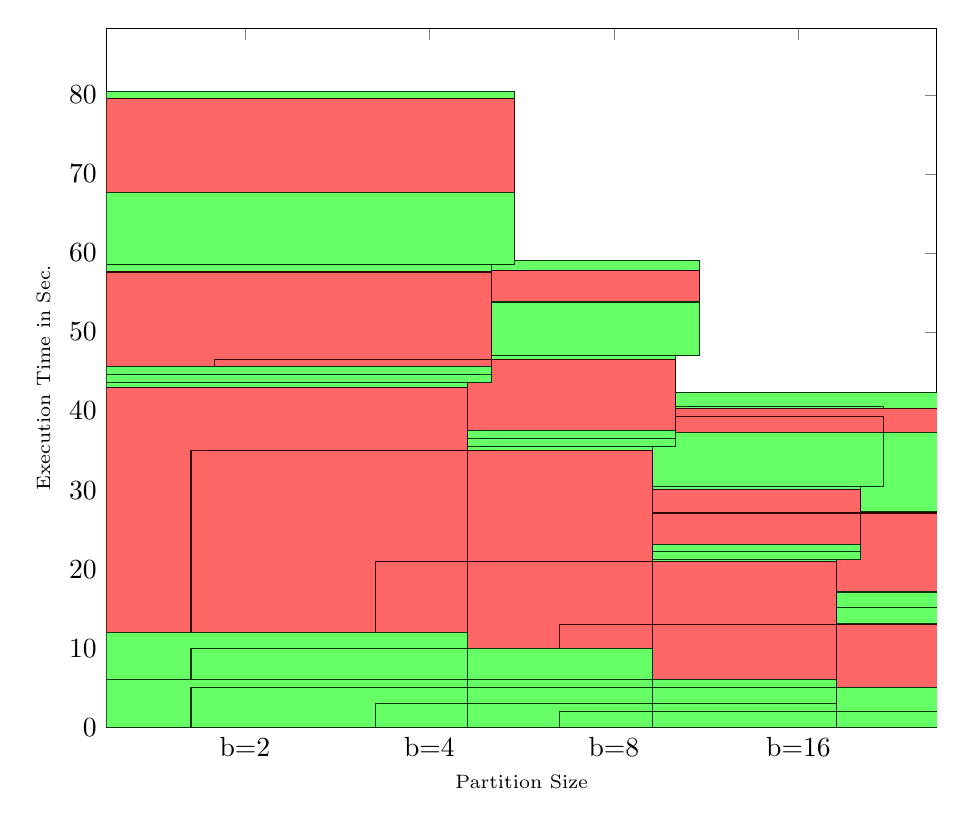
\begin{tikzpicture}
\begin{axis}[
width=\textwidth,
ybar stacked,bar width=5,
xtick={2,4,8,16},
ymin=0,
xmin=2, xmax=8,
enlarge x limits=0.25,
legend style={at={(1,1)},anchor=north west},
xlabel={\scriptsize Partition Size},
ylabel={\scriptsize Execution Time in Sec.},
xtick={2,4,6,8},
xticklabels={b=2,b=4,b=8,b=16},
%legend entries={A,B},
]
\addplot +[bar shift=-.1cm][green!20!black,fill=green!60!white] coordinates {(2,6) (4,5) (6,3) (8,2)};
\addplot +[bar shift=-.1cm][green!20!black,fill=green!60!white] coordinates {(2,6) (4,5) (6,3) (8,3)};
\addplot +[bar shift=-.1cm][red!20!black,fill=red!60!white] coordinates {(2,31) (4,25) (6,15) (8,8)};
\addplot +[bar shift=-.1cm][green!20!black,fill=green!60!white] coordinates {(2,0.6) (4,0.5) (6,0.2) (8,0.1)};

\resetstackedplots

\addplot +[bar shift=.2cm][green!20!black,fill=green!60!white] coordinates {(2,1) (4,1) (6,1) (8,2)};
\addplot +[bar shift=.2cm][green!20!black,fill=green!60!white] coordinates {(2,1) (4,1) (6,0.9) (8,2)};
\addplot +[bar shift=.2cm][red!20!black,fill=red!60!white] coordinates {(2,12) (4,9) (6,7) (8,10)};
\addplot +[bar shift=.2cm][green!20!black,fill=green!60!white] coordinates {(2,1) (4,0.5) (6,0.3) (8,0.2)};

\resetstackedplots

%\addplot +[bar shift=.5cm] coordinates {(2,9) (4,6.8) (6,6.9) (8,10)};
\addplot +[bar shift=.5cm][green!20!black,fill=green!60!white] coordinates {(2,9) (4,6.8) (6,6.9) (8,10)};
\addplot +[bar shift=.5cm][red!20!black,fill=red!60!white] coordinates {(2,12) (4,4) (6,2) (8,3)};
\addplot +[bar shift=.5cm][green!20!black,fill=green!60!white] coordinates {(2,0.8) (4,1.2) (6,1.3) (8,2.1)};
\end{axis}
\end{tikzpicture}
\end{subfigure}%
\begin{subfigure}[t]{.5\textwidth}
	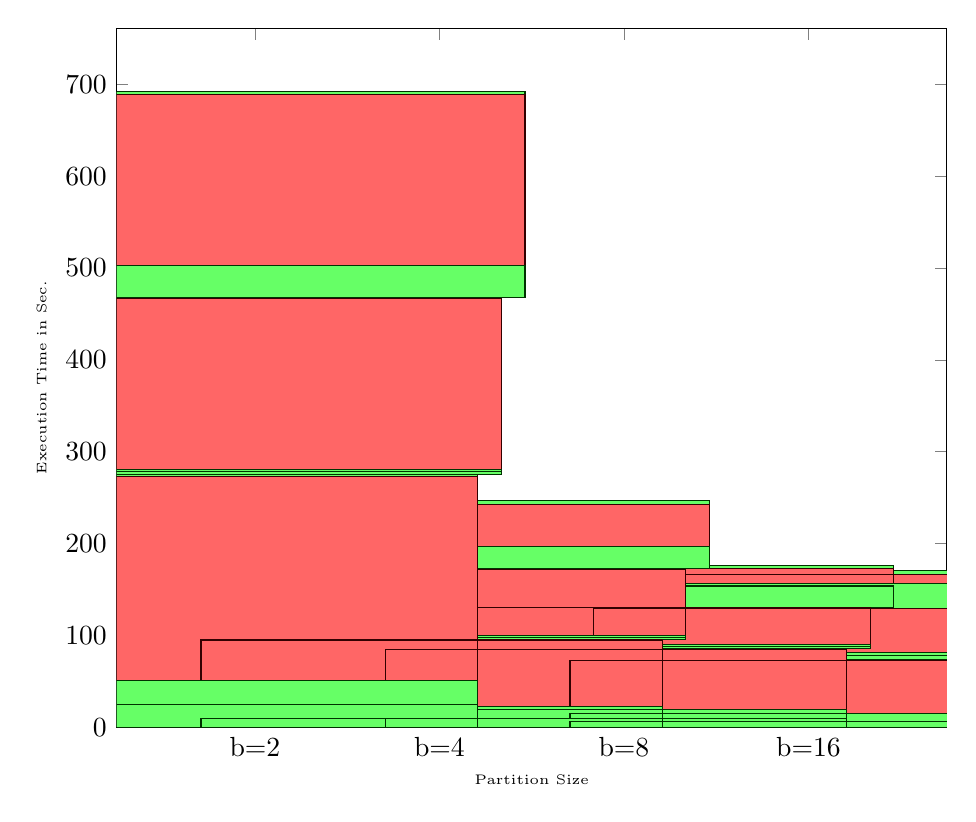
\begin{tikzpicture}
	\begin{axis}[
	width=\textwidth,
	ybar stacked,bar width=5,
	xtick={2,4,8,16},
	ymin=0,
	xmin=2, xmax=8,
	enlarge x limits=0.25,
	legend style={at={(1,1)},anchor=north west},
	xlabel={\tiny Partition Size},
	ylabel={\tiny Execution Time in Sec.},
	xtick={2,4,6,8},
	xticklabels={b=2,b=4,b=8,b=16},
	%legend entries={A,B},
	]
	\addplot +[bar shift=-.1cm][green!20!black,fill=green!60!white] coordinates {(2,25) (4,9) (6,9) (8,6)};
	\addplot +[bar shift=-.1cm][green!20!black,fill=green!60!white] coordinates {(2,26) (4,14) (6,10) (8,9)};
	\addplot +[bar shift=-.1cm][red!20!black,fill=red!60!white] coordinates {(2,222) (4,72) (6,66) (8,58)};
	\addplot +[bar shift=-.1cm][green!20!black,fill=green!60!white] coordinates {(2,2) (4,0.6) (6,0.3) (8,0.2)};
	\resetstackedplots
	\addplot +[bar shift=.2cm][green!20!black,fill=green!60!white] coordinates {(2,3) (4,2) (6,3) (8,5)};
	\addplot +[bar shift=.2cm][green!20!black,fill=green!60!white] coordinates {(2,3) (4,2) (6,2) (8,3)};
	\addplot +[bar shift=.2cm][red!20!black,fill=red!60!white] coordinates {(2,186) (4,72) (6,40) (8,48)};
	\addplot +[bar shift=.2cm][green!20!black,fill=green!60!white] coordinates {(2,1) (4,1) (6,0.4) (8,0.3)};
	\resetstackedplots
	%\addplot +[bar shift=.5cm] coordinates {(2,29) (4,15) (6,12) (8,12)};
	\addplot +[bar shift=.5cm][green!20!black,fill=green!60!white] coordinates {(2,35) (4,24) (6,23) (8,27)};
	\addplot +[bar shift=.5cm][red!20!black,fill=red!60!white] coordinates {(2,186) (4,46) (6,19) (8,10)};
	\addplot +[bar shift=.5cm][green!20!black,fill=green!60!white] coordinates {(2,3) (4,4) (6,3) (8,3.8)};
	\end{axis}
	\end{tikzpicture}
\end{subfigure}%

\begin{subfigure}[t]{.5\textwidth}
	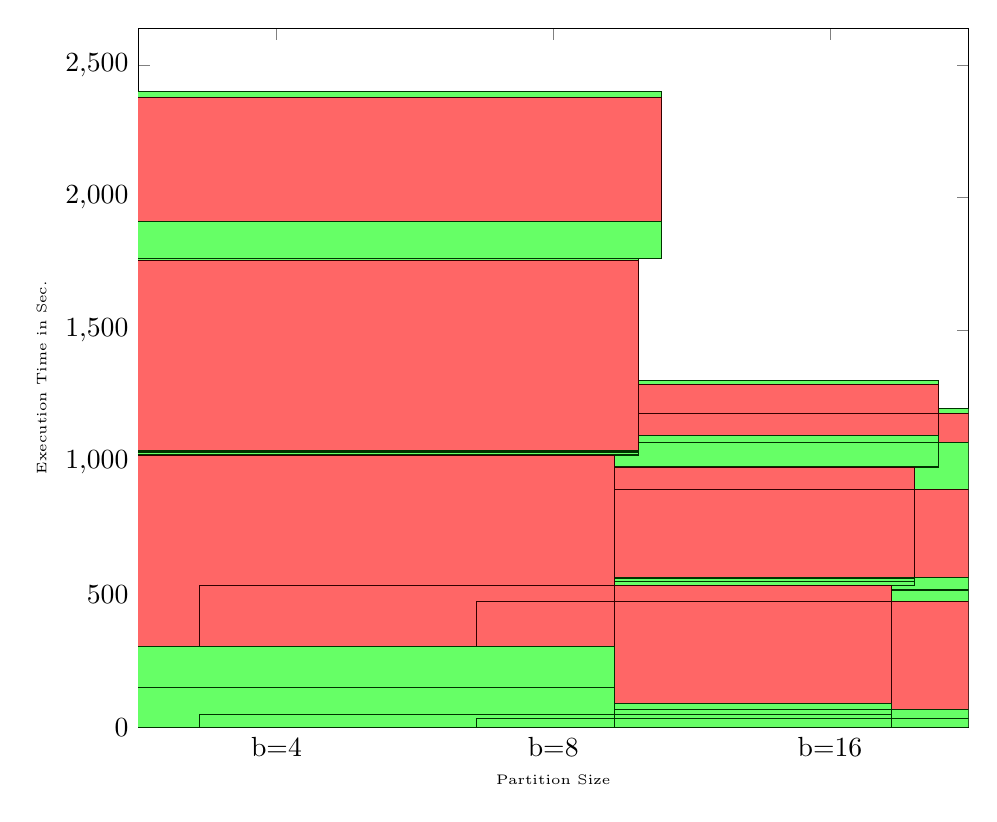
\begin{tikzpicture}
	\begin{axis}[
	width=\textwidth,
	ybar stacked,bar width=5,
	xtick={4,8,16},
	ymin=0,
	xmin=4, xmax=8,
	enlarge x limits=0.25,
	legend style={at={(1,1)},anchor=north west},
	xlabel={\tiny Partition Size},
	ylabel={\tiny Execution Time in Sec.},
	xtick={4,6,8},
	xticklabels={b=4,b=8,b=16},
	%legend entries={A,B},
	]
	\addplot +[bar shift=-.1cm][green!20!black,fill=green!60!white] coordinates {(4,150) (6,49) (8,33)};
	\addplot +[bar shift=-.1cm][green!20!black,fill=green!60!white] coordinates {(4,156) (6,42) (8,34)};
	\addplot +[bar shift=-.1cm][red!20!black,fill=red!60!white] coordinates {(4,720) (6,444) (8,408)};
	\addplot +[bar shift=-.1cm][green!20!black,fill=green!60!white] coordinates {(4,2) (6,0.5) (8,0.2)};
	
	\resetstackedplots
	
	\addplot +[bar shift=.2cm][green!20!black,fill=green!60!white] coordinates {(4,9) (6,14) (8,43)};
	\addplot +[bar shift=.2cm][green!20!black,fill=green!60!white] coordinates {(4,6) (6,12) (8,48)};
	\addplot +[bar shift=.2cm][red!20!black,fill=red!60!white] coordinates {(4,720) (6,420) (8,330)};
	\addplot +[bar shift=.2cm][green!20!black,fill=green!60!white] coordinates {(4,6) (6,1) (8,1)};
	
	\resetstackedplots
	
	%\addplot +[bar shift=.5cm][green!20!black,fill=green!60!white] coordinates {(4,90) (6,48) (8,43)};
	\addplot +[bar shift=.5cm][green!20!black,fill=green!60!white] coordinates {(4,140) (6,119) (8,179)};
	\addplot +[bar shift=.5cm][red!20!black,fill=red!60!white] coordinates {(4,470) (6,192) (8,108)};
	\addplot +[bar shift=.5cm][green!20!black,fill=green!60!white] coordinates {(4,21) (6,15) (8,18)};
	
	
	\end{axis}
	\end{tikzpicture}
\end{subfigure}%
\caption{Comparing stage-wise running time of MLLib, Marlin and Stark for matrix size $(4096\times 4096)$, $(8192\times 8192)$, $(16384\times 16384)$ for increasing partition Size}\label{fig:Stagewise}
\end{figure}

\begin{table}[h!]
	\caption{Stage-wise performance comparison of three systems with increasing partition (The unit of execution time is second) for matrix size $4096\times 4096$}
	\label{tab:Stagewise-4096}
	\begin{minipage}{\columnwidth}
		\begin{center}
			\begin{tabular}{lllllllllllll}
				\toprule
				Stage & \multicolumn{12}{c}{Execution Time} \\
				& \multicolumn{3}{c}{b=2} & \multicolumn{3}{c}{b=4} & \multicolumn{3}{c}{b=8} & \multicolumn{3}{c}{b=16} \\
				& M1 & M2 & S & M1 & M2 & S & M1 & M2 & S & M1 & M2 & S \\	
				\toprule			
				Stage 1 & \cellcolor{green}6 & \cellcolor{green}1 & 8 & \cellcolor{green}5 & \cellcolor{green}1 & 4 & \cellcolor{green}3 & \cellcolor{green}1 & 4 & \cellcolor{green}2 & \cellcolor{green}2 & 4 \\				
				\toprule				
				Stage 2 & \cellcolor{green}6 & \cellcolor{green}1 & \cellcolor{green}1 & \cellcolor{green}5 & \cellcolor{green}1 & \cellcolor{green}2 & \cellcolor{green}3 & \cellcolor{green}0.9 & \cellcolor{green}1 & \cellcolor{green}3 & \cellcolor{green}2 & \cellcolor{green}1 \\
				\toprule
				Stage 3 & \cellcolor{red}31 & \cellcolor{red}12 & \cellcolor{red}12 & \cellcolor{red}25 & \cellcolor{red}9 & \cellcolor{green}0.8 & \cellcolor{red}15 & \cellcolor{red}7 & \cellcolor{green}1 & \cellcolor{red}8 & \cellcolor{red}10 & \cellcolor{green}1 \\
				\toprule
				Stage 4 & \cellcolor{green}0.6 & \cellcolor{green}1 & \cellcolor{green}0.8 & \cellcolor{green}0.5 & \cellcolor{green}0.5 & \cellcolor{red}4 & \cellcolor{green}0.2 & \cellcolor{green}0.3 & \cellcolor{green}0.9 & \cellcolor{green}0.1 & \cellcolor{green}0.2 & \cellcolor{green}2 \\
				\toprule
				Stage 5 & & & & & & \cellcolor{green}0.5 & & & \cellcolor{red}2 & & & \cellcolor{green}2 \\
				\toprule			
				Stage 6 & & & & & & \cellcolor{green}0.7 & & & \cellcolor{green}0.5 & & & \cellcolor{red}3 \\
				\toprule
				Stage 7 & & & & & & & & & \cellcolor{green}0.5 & & & \cellcolor{green}0.9 \\
				\toprule
				Stage 8 & & & & & & & & & \cellcolor{green}0.3 & & & \cellcolor{green}0.5 \\
				\toprule
				Stage 9 & & & & & & & & & & & & \cellcolor{green}0.4 \\
				\toprule
				Stage 10 & & & & & & & & & & & & \cellcolor{green}0.3 \\
				\bottomrule
			\end{tabular}
		\end{center}
	\end{minipage}
\end{table}

\begin{table}[h!]
	\caption{Stage-wise performance comparison of three systems with increasing partition (The unit of execution time is second) for matrix size $8192\times 8192$}
	\label{tab:Stagewise-8192}
	\begin{minipage}{\columnwidth}
		\begin{center}
			\begin{tabular}{lllllllllllll}
				\toprule
				Stage & \multicolumn{12}{c}{Execution Time} \\
				& \multicolumn{3}{c}{b=2} & \multicolumn{3}{c}{b=4} & \multicolumn{3}{c}{b=8} & \multicolumn{3}{c}{b=16} \\
				& M1 & M2 & S & M1 & M2 & S & M1 & M2 & S & M1 & M2 & S \\	
				\toprule			
				Stage 1 & \cellcolor{green}25 & \cellcolor{green}3 & 29 & \cellcolor{green}9 & \cellcolor{green}2 & 15 & \cellcolor{green}9 & \cellcolor{green}3 & 12 & \cellcolor{green}6 & \cellcolor{green}5 & 12 \\				
				\toprule				
				Stage 2 & \cellcolor{green}26 & \cellcolor{green}3 & \cellcolor{green}6 & \cellcolor{green}14 & \cellcolor{green}2 & \cellcolor{green}6 & \cellcolor{green}10 & \cellcolor{green}2 & \cellcolor{green}4 & \cellcolor{green}9 & \cellcolor{green}3 & \cellcolor{green}4 \\
				\toprule
				Stage 3 & \cellcolor{red}222 & \cellcolor{red}186 & \cellcolor{red}186 & \cellcolor{red}72 & \cellcolor{red}72 & \cellcolor{green}3 & \cellcolor{red}66 & \cellcolor{red}40 & \cellcolor{green}4 & \cellcolor{red}58 & \cellcolor{red}48 & \cellcolor{green}3 \\
				\toprule
				Stage 4 & \cellcolor{green}2 & \cellcolor{green}1 & \cellcolor{green}3 & \cellcolor{green}0.6 & \cellcolor{green}1 & \cellcolor{red}46 & \cellcolor{green}0.3 & \cellcolor{green}0.4 & \cellcolor{green}3 & \cellcolor{green}0.2 & \cellcolor{green}0.3 & \cellcolor{green}4 \\
				\toprule
				Stage 5 & & & & & & \cellcolor{green}2 & & & \cellcolor{red}19 & & & \cellcolor{green}4 \\
				\toprule			
				Stage 6 & & & & & & \cellcolor{green}2 & & & \cellcolor{green}1 & & & \cellcolor{red}10 \\
				\toprule
				Stage 7 & & & & & & & & & \cellcolor{green}1 & & & \cellcolor{green}1 \\
				\toprule
				Stage 8 & & & & & & & & & \cellcolor{green}1 & & & \cellcolor{green}0.9 \\
				\toprule
				Stage 9 & & & & & & & & & & & & \cellcolor{green}0.9 \\
				\toprule
				Stage 10 & & & & & & & & & & & & \cellcolor{green}1 \\
				\bottomrule
			\end{tabular}
		\end{center}
	\end{minipage}
\end{table}

\begin{table}[h!]
	\caption{Stage-wise performance comparison of three systems with increasing partition (The unit of execution time is second) for matrix size $16384\times 16384$}
	\label{tab:Stagewise-16384}
	\begin{minipage}{\columnwidth}
		\begin{center}
			\begin{tabular}{llllllllll}
				\toprule
				Stage & \multicolumn{9}{c}{Execution Time} \\
				& \multicolumn{3}{c}{b=4} & \multicolumn{3}{c}{b=8} & \multicolumn{3}{c}{b=16} \\
				& M1 & M2 & S & M1 & M2 & S & M1 & M2 & S \\	
				\toprule			
				Stage 1 & \cellcolor{green}150 & \cellcolor{green}9 & 90 &  \cellcolor{green}49 & \cellcolor{green}14 & 48 & \cellcolor{green}33 & \cellcolor{green}43 & 43\\				
				\toprule			
				Stage 2 & \cellcolor{green}156 & \cellcolor{green}6 & \cellcolor{green}37 & \cellcolor{green}42 & \cellcolor{green}12 & \cellcolor{green}26 & \cellcolor{green}34 & \cellcolor{green}48 & \cellcolor{green}36\\
				\toprule
				Stage 3 & \cellcolor{red}720 & \cellcolor{red}720 & \cellcolor{green}13 & \cellcolor{red}444 & \cellcolor{red}420 & \cellcolor{green}24 & \cellcolor{red}408 & \cellcolor{red}330 & \cellcolor{green}21\\
				\toprule
				Stage 4 & \cellcolor{green}2 & \cellcolor{green}6 & \cellcolor{red}470 & \cellcolor{green}0.5 & \cellcolor{green}1 & \cellcolor{green}21 & \cellcolor{green}0.2 & \cellcolor{green}1 & \cellcolor{green}46\\
				\toprule
				Stage 5 &  & & \cellcolor{green}9 &  &  & \cellcolor{red}192 & &  & \cellcolor{green}33\\
				\toprule			
				Stage 6 &  &  & \cellcolor{green}12 &  &  & \cellcolor{green}4 & &  & \cellcolor{red}108\\
				\toprule
				Stage 7 &  &  & &  &  & \cellcolor{green}6 & &  & \cellcolor{green}6\\
				\toprule
				Stage 8 &  &  & &  &  & \cellcolor{green}5 & &  & \cellcolor{green}3\\
				\toprule
				Stage 9 &  &  & &  &  &   & &  & \cellcolor{green}4\\
				\toprule
				Stage 10 &  & & &  &  &   & &  & \cellcolor{green}5\\
				\bottomrule
			\end{tabular}
		\end{center}
	\end{minipage}
\end{table}

\subsection{Scalability}
In this section, we investigate the scalability of \textit{Stark}. For this, we generate three test cases, each containing a different set of two matrices of dimensions equal to $(4096\times 4096)$, $(8192\times 8192)$ and $(16384\times 16384)$. The running time vs. the number of spark executors for these $3$ pairs of matrices is shown in Fig. \ref{fig:scale}. The ideal scalability line (i.e. $T(n) = T(1)/n$ - where $n$ is the number of executors) has been over-plotted on this figure in order to demonstrate the scalability of our algorithm. We can see that \textit{Stark} has a very good strong scalability, with a minor deviation from ideal scalability when the size of the matrix is low (i.e. for $(8192\times 8192)$ and $(16384\times 16384)$).  

\begin{figure}[!ht]
	\begin{subfigure}[t]{.35\textwidth}
		\begin{tikzpicture}
		\begin{axis}[
		xmin=0,
		xmax=6,
		xtick={1,2,3,4,5},
		ytick={4,8,12,16,20,24},
		x tick label style={/pgf/number format/1000 sep=},
		xlabel={\tiny Number of Executors},
		ylabel={\tiny Execution Time in Sec.},
		legend style={at={(0.38,1.4)},anchor=north},
		width=\textwidth,
		]
		\addplot coordinates {(1,21.5) (2,10.75) (3,7.16) (4,5.37) (5,4.3)};
		\addlegendentry{\tiny Ideal}
		\addplot coordinates {(1,21.5) (2,14) (3,10.8) (4,10.8) (5,9.5)};
		\addlegendentry{\tiny Experimental}
		\end{axis}
		\end{tikzpicture}
		\caption{$4096\times 4096$},
	\end{subfigure}%
	\begin{subfigure}[t]{.35\textwidth}
		\begin{tikzpicture}
		\begin{axis}[
		xmin=0,
		xmax=6,
		xtick={1,2,3,4,5},
		ytick={25,50,75,100,125,150,175,200},
		x tick label style={/pgf/number format/1000 sep=},
		xlabel={\tiny Number of Executors},
		ylabel={\tiny Execution Time in Sec.},
		legend style={at={(0.38,1.4)},anchor=north},
		width=\textwidth,
		]
		\addplot coordinates {(1,114.6) (2,57.3) (3,38.2) (4,28.65) (5,22.92)};
		\addlegendentry{\tiny Ideal}
		\addplot coordinates {(1,114.6) (2,66.6) (3,50.7) (4,46.4) (5,40.6)};
		\addlegendentry{\tiny Experimental}
		\end{axis}
		\end{tikzpicture}
		\caption{$8192\times 8192$}
	\end{subfigure}%
	\begin{subfigure}[t]{.35\textwidth}
		\begin{tikzpicture}
		\begin{axis}[
		xmin=0,
		xmax=6,
		xtick={1,2,3,4,5},
		ytick={250,500,750,1000,1250,1500},
		x tick label style={/pgf/number format/1000 sep=},
		xlabel={\tiny Number of Executors},
		ylabel={\tiny Execution Time in Sec.},
		legend style={at={(0.38,1.4)},anchor=north},
		width=\textwidth,
		]
		\addplot coordinates {(1,1525) (2,762.5) (3,508.33) (4,381.25) (5,305)};
		\addlegendentry{\tiny Ideal}
		\addplot coordinates {(1,1525) (2,763) (3,520) (4,410) (5,325)};
		\addlegendentry{\tiny Experimental}
		\end{axis}
		\end{tikzpicture}
		\caption{$16384\times 16384$}
	\end{subfigure}%
	\caption{The scalability of \textit{Stark}, in comparison with ideal scalability (blue line), on matrix $(4096\times 4096)$, $(8192\times 8192)$ and $(16384\times 16384)$}\label{fig:scale}
\end{figure}

%\subsection{Network}
%We measure the total amount of network traffic or shuffle in these three approaches. Here network refers to shuffle read which is the sum of read serialized data on all executors at the beginning of a stage. We sum all the shuffle read size for all the stages for a particular job and report that to compare with others. The experiments are conducted in a similar way as the experiments were conducted in efficiency analysis. we conducted two test cases. In the first test case, we make the partition size constant and with increasing matrix size we report the shuffle size. In the second test case, we generate shuffle with increasing partition size for constant matrix size.

%In the first test case, we generate four scenarios. In each scenario, we take partition size $b$ as 2, 4, 8 and 16 respectively and increase matrix size from $(4096\times 4096)$ to $(16384\times 16384)$. Figure \ref{fig:shuffle-read-partition} shows scenarios respectively.

%\begin{figure}[!h]
%	\begin{subfigure}[b]{0.4\textwidth}
%	\includegraphics[width=\linewidth]{images/Shuffle-Read-b16}
%	%\caption{A gull}
%	\label{fig:Shuffle-Read-b16}
%	\end{subfigure}%
%	\begin{subfigure}[b]{0.4\textwidth}
%	\includegraphics[width=\linewidth]{images/Shuffle-Read-b8}
%	%\caption{A gull2}
%	\label{fig:Shuffle-Read-b8}
%	\end{subfigure}
%	\centering
%	\begin{subfigure}[b]{0.4\textwidth}
%	\includegraphics[width=\linewidth]{images/Shuffle-Read-b4}
%	%\caption{A tiger}
%	\label{fig:Shuffle-Read-b4}
%	\end{subfigure}%
%	\caption{Comparing running time of Stark and Marlin for b = 16, b = 8 and b = 4 for increasing matrix size}\label{fig:shuffle-read-partition}
%\end{figure}

%In the second test case, we do the opposite. Here, we generate four scenarios as before. However, in each scenario, we take matrix size as $(4096\times 4096)$ to $(16384\times 16384)$ as constant, and increase the partition size $b$ from 2 to 16. Figure \ref{fig:shuffle-read} shows the scenarios respectively.

%\begin{figure}[!h]
%	\begin{subfigure}[b]{0.4\textwidth}
%	\includegraphics[width=\linewidth]{images/Shuffle-Read-4096}
%	%\caption{A gull}
%	\label{fig:Shuffle-Read-4096}
%	\end{subfigure}%
%	\begin{subfigure}[b]{0.4\textwidth}
%	\includegraphics[width=\linewidth]{images/Shuffle-Read-8192}
%	%\caption{A gull2}
%	\label{fig:Shuffle-Read-8192}
%	\end{subfigure}
%	\centering
%	\begin{subfigure}[b]{0.4\textwidth}
%	\includegraphics[width=\linewidth]{images/Shuffle-Read-16384}
%	%\caption{A tiger}
%	\label{fig:Shuffle-Read-16384}
%	\end{subfigure}%
%	\caption{Comparing shuffle read of Marlin, Stark and MLLib for matrix size $(4096\times 4096)$, $(8192\times 8192)$, $(16384\times 16384)$ for increasing partition size}\label{fig:shuffle-read}
%\end{figure}

\section{Conclusions and Future Work}
\label{sec:conclusion}
With \textit{Stark}, we developed an algorithm for MM which implemented Strassen's MM algorithm distributedly in a commodity cluster. \textit{Stark} provides a faster, scalable and massively parallel approach to multiply two large matrix in Spark compared to state-of-the-art \textit{MLLib} and \textit{Marlin}. It accomplishes that using creating a recursive tree of computation and performing parallel computation on each node of a level of that tree. Additionally, it tags the block matrices intelligently to memorize them in the subsequent recursive calls. Our theoretical analysis shed light on the time consuming stages of the competing approaches and experimental results matches with the earlier. The experimental results show that the scalability of \textit{Stark} becomes highly robust when matrix size is increased.

The next step from the practical side are experiments with massive matrix sizes (for example, $2^{17}\times 2^{17}$ using more number of nodes and executors. On the theoretical side, we could look for faster efficient multiplication algorithm such as Winograd variation \cite{coppersmith1990matrix} of Strassen's MM algorithm. In future, we will look into implementing Strassen's and Winograd variation on rectangular matrices.   


%In this article, we develop the first multifrequency MAC protocol for
%WSN applications in which each device adopts a
%single radio transceiver. The different MAC design requirements for
%WSNs and general wireless ad-hoc networks are
%compared, and a complete WSN multifrequency MAC design (MMSN) is
%put forth. During the MMSN design, we analyze and evaluate different
%choices for frequency assignments and also discuss the nonuniform
%back-off algorithms for the slotted media access design.

% Start of "Sample References" section

%\section{Typical references in new ACM Reference Format}
%A paginated journal article \cite{Abril07}, an enumerated
%journal article \cite{Cohen07}, a reference to an entire issue \cite{JCohen96},
%a monograph (whole book) \cite{Kosiur01}, a monograph/whole book in a series (see 2a in spec. document)
%\cite{Harel79}, a divisible-book such as an anthology or compilation \cite{Editor00}
%followed by the same example, however we only output the series if the volume number is given
%\cite{Editor00a} (so Editor00a's series should NOT be present since it has no vol. no.),
%a chapter in a divisible book \cite{Spector90}, a chapter in a divisible book
%in a series \cite{Douglass98}, a multi-volume work as book \cite{Knuth97},
%an article in a proceedings (of a conference, symposium, workshop for example)
%(paginated proceedings article) \cite{Andler79}, a proceedings article
%with all possible elements \cite{Smith10}, an example of an enumerated
%proceedings article \cite{VanGundy07},
%an informally published work \cite{Harel78}, a doctoral dissertation \cite{Clarkson85},
%a master's thesis: \cite{anisi03}, an online document / world wide web
%resource \cite{Thornburg01, Ablamowicz07, Poker06}, a video game (Case 1) \cite{Obama08} and (Case 2) \cite{Novak03}
%and \cite{Lee05} and (Case 3) a patent \cite{JoeScientist001},
%work accepted for publication \cite{rous08}, 'YYYYb'-test for prolific author
%\cite{SaeediMEJ10} and \cite{SaeediJETC10}. Other cites might contain
%'duplicate' DOI and URLs (some SIAM articles) \cite{Kirschmer:2010:AEI:1958016.1958018}.
%Boris / Barbara Beeton: multi-volume works as books
%\cite{MR781536} and \cite{MR781537}.

%A couple of citations with DOIs: \cite{2004:ITE:1009386.1010128,
%  Kirschmer:2010:AEI:1958016.1958018}. 

% Appendix


% Bibliography
\bibliographystyle{ACM-Reference-Format}
\bibliography{sample-bibliography}
